\documentclass[11pt]{article}

\usepackage{graphicx}
\usepackage{hyperref}
\usepackage{xcolor}
\usepackage{float}
\usepackage{fancyvrb}
\usepackage{amsmath}
\usepackage{amssymb}
\usepackage[margin=0.70in]{geometry}
\usepackage[ruled,vlined]{algorithm2e}
\usepackage{subcaption}
\usepackage{spverbatim}
\usepackage[mathletters]{ucs}
\usepackage[utf8x]{inputenc}
\usepackage{fancyhdr}
\usepackage{enumitem}

\pagestyle{fancy}
\fancyhf{}
\rhead{Giulio Serra 1904089, Matteo Salvino 1708108}
\lhead{AD 20/21}

\fvset{tabsize=4}

\iffalse
\title{%
  Algorithm Design \\
  \large 2020-2021}

\author{Giulio Serra - Matteo Salvino}
\date{January 10, 2020}
\fi

\graphicspath{ {images/} }

\newenvironment{claim}[1]{\par\textbf{Claim}\space#1}{}
\newenvironment{proof}[1]{\par\textit{Proof}\space#1}{\hfill\ensuremath{\square}}

\begin{document}
\tableofcontents
%\maketitle
%\pagebreak
%\tableofcontents
%\pagebreak

\section{Stable Matching}
The stable matching solves the problem of assigning one element $x \in X$ to another element $y \in Y$(for example: men to wimen, intern to hospitals, ecc...).

\begin{itemize}
\item Unstable Pairs\\
A pair p(x,y) is defined as unstable if $\exists y^{*} \in Y \; such \;that \;p(x,y^{*}) > p(x,y) \; and \; vice-versa. $ 

\item Stable Matching\\
A matching containing no unstable pairs.
\end{itemize}


\begin{figure}[h]
		\centering
		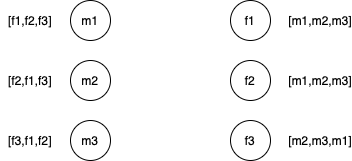
\includegraphics[width=0.4\textwidth ]{GS}
		\caption{An instance of the problem containing the M and W sets and $\forall m \in M, \; \forall w \in W$ a list of preferences for the elements in the opposite set, in increasing order.}
\end{figure}

\begin{figure}[h]
		\centering
		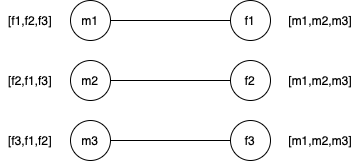
\includegraphics[width=0.4\textwidth ]{GS-Solved}
		\caption{A solution for the instance of the problem, containing only stable pairs.}
\end{figure}


\subsection{The Men-Wimen problem}
The problem about finding the stable matching between a set W and M. Each $w \in W$ rank every $m \in M$ from best to worst, and every $m \in M$ do the same.

\begin{algorithm}[H]
\SetAlgoLined
\small
\KwIn{$M$ set of men, $W$ set of women}
\KwOut{$S$ the set containing all the stable pairs between M and W}
\BlankLine

$S \leftarrow$ set containing all the pairs between M and W.

\BlankLine
\While{$\exists m \in M$ that is free and haven't proposed yet}{
    $w_{i} = m[0] \leftarrow$ first woman in m's list of preference to whom he is not yet proposed \; 
     \If{$w_{i} \; is \; free$}{
     	$S = S \cup p(m,w_{i}) \leftarrow$ create a pair between m and $w_{i}$\;
     }{
      }
      \BlankLine
        \If{$w_{i}$ prefers m to her current partner $m_{i}$}{
        	 $S = S - p(m_{i},w_{i})$\;
     	  $S = S \cup p(m,w_{i})$\;

     }{
      }
      \BlankLine
    
}
\BlankLine

return $S$\;
\caption{proposeAndReject(M, W) :}
\end{algorithm} 

\begin{itemize}
\item Observation 1\\
Every men propose to a women decreasing order of preference, for every women is the opposite. 

\item Observation 2\\
Once a women is matched she never become un-matched, she just change her partner, in increasing order of preference.

\item Observation 3\\
Assuming $|M| = |W|$ then the algorithm has $\mathcal{O}(n^{2})$ complexity.

\item Observation 4\\
The algorithm is very resistant to modifications: example new conditions on engagements.
\end{itemize}

\clearpage

\section{Asymptotic Order of Growth}

\subsection{Brute Force}
For many non-trivial problems, there is a natural brute force search algorithm that checks every possible solution, usually taking $2^{n}$.
\subsection{Polynomial Running Time}
This is the most desirable running time of any algorithm because it scales with ease at the increment of the input size.\\An algorithm can be defined as poly-time if the following property holds:

\[ \exists c > 0, \exists d >0, \; such \; that \; \forall n \in INPUT \; the \; running \; time \; is \; bounded \; by\; cn^{d} \]

We can now give the following definition of efficiency:

\[ An \; algorithm \; is \; efficient \; if \; it \; is \; poly-time.\]

When discussing the running time of a deterministic algorithm is important to take into account the worst-case scenario because, in doing that, the running time is guaranteed $\forall n \in INPUT.$ There are some exception to this rule, when the worst-case scenario is very rare.\\\\
When discussing of probabilistic algorithm we need, instead, to reason upon the expected running time.

\subsection{Big-O Notation}

Assuming we have an algorithm rappresented by the function:
 \[ T(n) = 1.6n^{2} + 3.5n+8\]
 We want a way to express the growing rate in a way that is insensitive to constant factors and low-ordered terms, in fact It can be said that T(n) grows like $\mathcal{O}(n^{2})$.\\

\begin{itemize}
\item The lower bound $\mathcal{O}$\\
We can say that T(n) is $\mathcal{O}{(f(n))}$ if $\exists c > 0, \exists n_{0} \geq 0 / \; T(n) \leq cf(n), \; \forall n \geq n_{0}$

We can give an alternative definition as follow:
 \[ \mathcal{O}{(f(n))} = \lim_{n\to\infty} \frac{T(n)}{F(n)} < \infty\]
 
Graphically:

\begin{figure}[H]
		\centering
		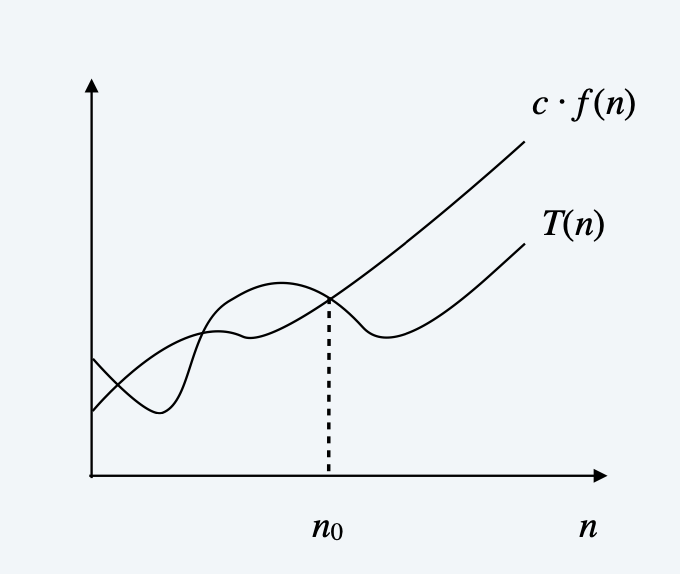
\includegraphics[width=0.4\textwidth ]{on}
\end{figure}

Again, going back to our function: $T(n) = 1.6n^{2} + 3.5n+8$, 
\[ T(n) = n^{3}\]
\[ T(n) = n^{2}\]
\[ T(n) \neq n\]


\item The upper bound $\Omega$ \\
We can say that T(n) is $ \Omega(f(n)) \;if \exists c > 0, \exists n_{0} \geq 0 / \; T(n) \geq cf(n), \; \forall n \geq n_{0}$

Again, going back to our function: $T(n) = 1.6n^{2} + 3.5n+8$, 
\[ T(n) = \Omega(n)\]
since $T(n) \leq pn^{2} \leq pn$.\\


Graphically:

\begin{figure}[H]
		\centering
		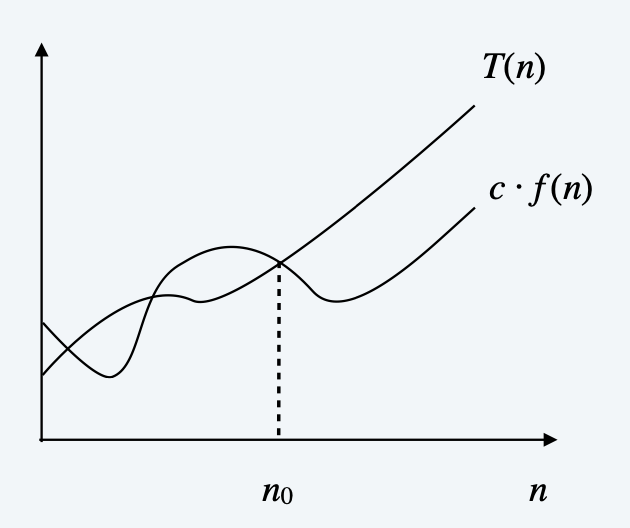
\includegraphics[width=0.4\textwidth ]{omega}
\end{figure}

\item The tight bound $\Theta$ \\
T(n) is $ \Theta(f(n)) \; if \; \exists c_{1} > 0, c_{2}>0 \; and \; \nexists \;n_{0} \; such \; that \; c_{1}f(n) \leq T(n) \leq c_{2} f(n) \; \forall n \geq n_{0}$

Graphically:

\begin{figure}[H]
		\centering
		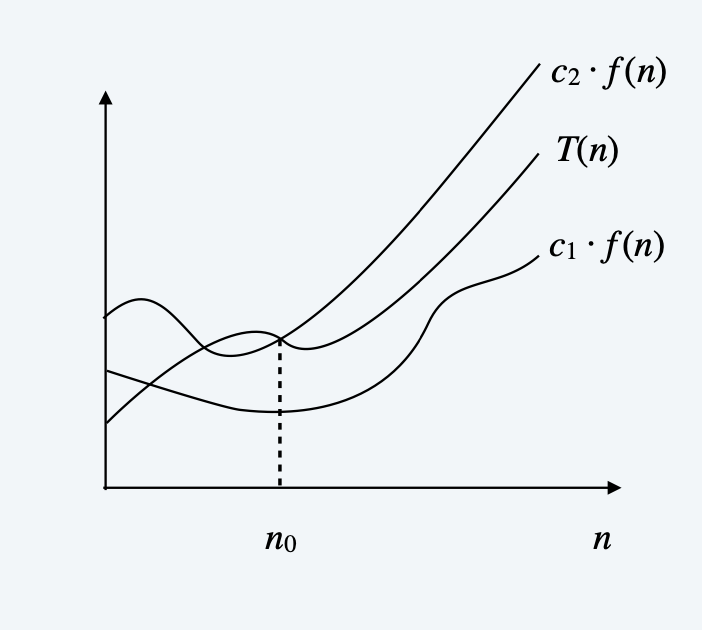
\includegraphics[width=0.4\textwidth ]{tight}
\end{figure}

\item {Usefull Properties}\\\\
Transitivity:
\[ if \; f = \mathcal{O}{(g)} \; and \; g =\mathcal{O}{(h)}, \; then \;f = \mathcal{O}{(h)}\]
\[ if \; f = \Omega{(g)} \; and \; g =\Omega{(h)}, \; then \;f = \Omega{(h)}\]\\\\
Sum of functions:
Supposing that f and g are two functions such that, for some other function h, we have $f = \mathcal{O}{(h)} \; and \;g = \mathcal{O}{(h)}, \; then \; f + g = \mathcal{O}{(h)}.$

\end{itemize}

\subsection{Common Running Times}

\begin{itemize}

\item {Linear $\mathcal{O}{(n)}$}\\\\
The running time is proportional to the input size.\\\\
Example: finding the maximum into an array.

\item {Linearithmic time $\mathcal{O}{(nlogn)}$}\\\\
Very common in divide-and-conquer algorithms, is also the running time of most of the sorting algorithms (ex: MergeSort or HeapSort).\\\\
Note: if an algorithm A execute n times a sorting operation, let's say n=3, and the sorting operation is still the most computational costly operation in the whole algorithm: then A is still $\mathcal{O}{(nlogn)}$ because $3\mathcal{O}{(nlogn)} \simeq \mathcal {O}{(nlogn)}$.

\item {Quadratic time $\mathcal{O}{(n^{2})}$}\\\\
Common when enumerating all pairs of elements, ex: given a list of n points in the plane $(x_{1}, y_{1})$, ..., $(x_{n}, y_{n})$, find the pair that is closest to each other.

\item {Cubic time $\mathcal{O}{(n^{3})}$}\\\\
Example:Set disjointness. Given n sets: $S_{1}, ..., S_{n}$ each of which is a subset of 1, 2, ..., n, is there some pair of these which are disjoint?

\item {Ploynomial time $\mathcal{O}{(n^{k})}$}\\\\
Example:Independent set of size k: Given a graph, are there k nodes such that no two are joined by an edge? The solution is to enumerate all subsets of k nodes.

\item {Exponential time}\\\\
Given a graph, what is maximum cardinality of an independent set? Enumerate all the possible subsets $\Rightarrow \mathcal{O}{(n^{2} 2n)}$

\item {Sublinear time}\\\\
Search in a sorted array. Given a sorted array A of n numbers, is a given number x in the array? $ \Rightarrow \mathcal{O}{(logn)}$ Binary search.

\subsection{Why it Matters}

\begin{figure}[H]
		\centering
		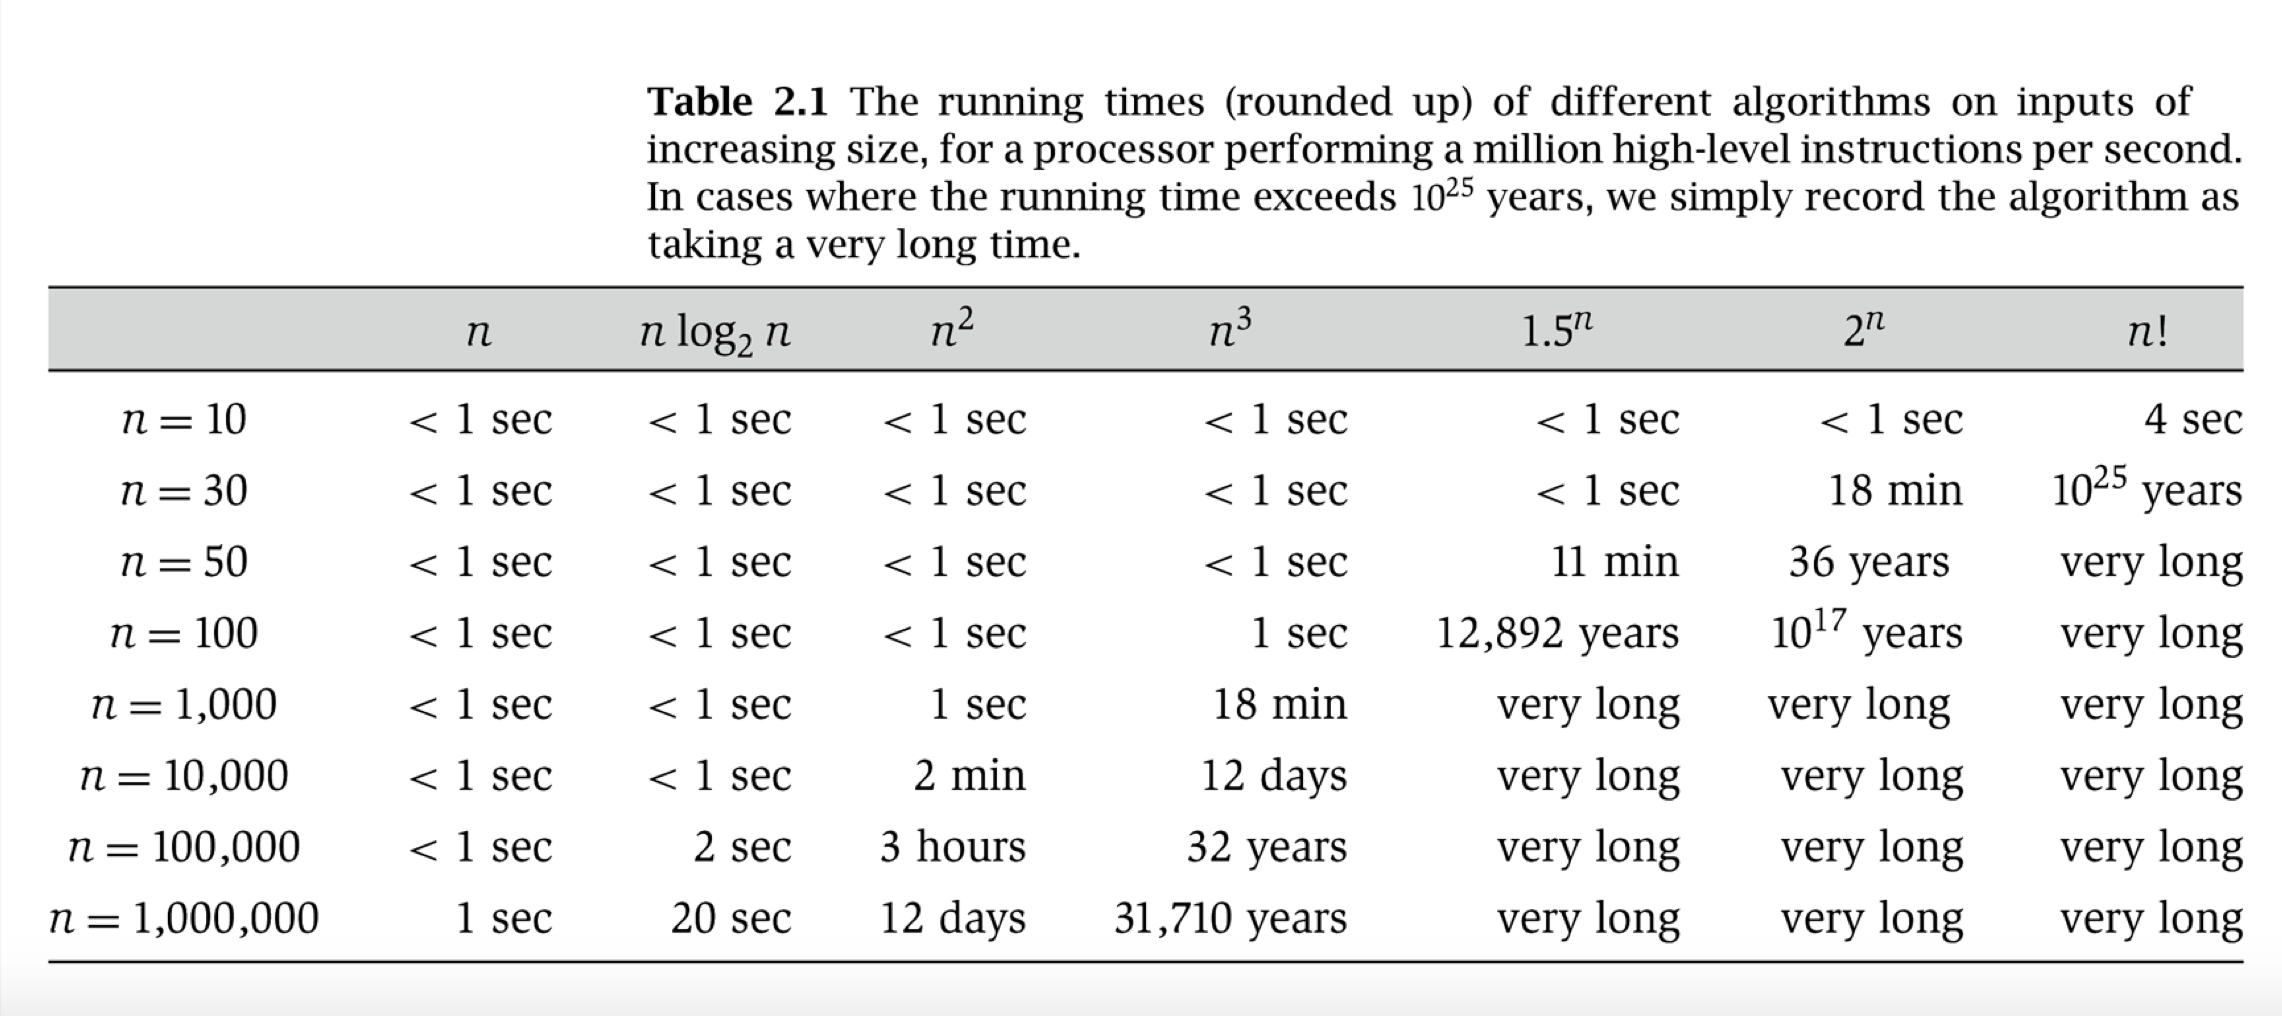
\includegraphics[width=0.7\textwidth ]{running}
		\caption{Comparison of the running times of different complexity algorithms.}
\end{figure}

Notice that, as we distance from the linear complexity, for bigger value of $n \in INPUT$, the execution time goes very high, this is bad: let's just say we want to deploy our non-linear algorithm on a distributed system dealing with a lots of records, as they grows, the system could become unable to process them in a feasible time.

\subsection{The Heap Data Structure}

Is a balanced binary tree  T(V,E) that satisfy the following property, defining with C the set containing all the children of a node $w_{i}$

\[ \forall w_{i} \in V, \forall v_{i} \in C, \; key(w_{i}) \leq key(v_{i})\]

\begin{figure}[H]
		\centering
		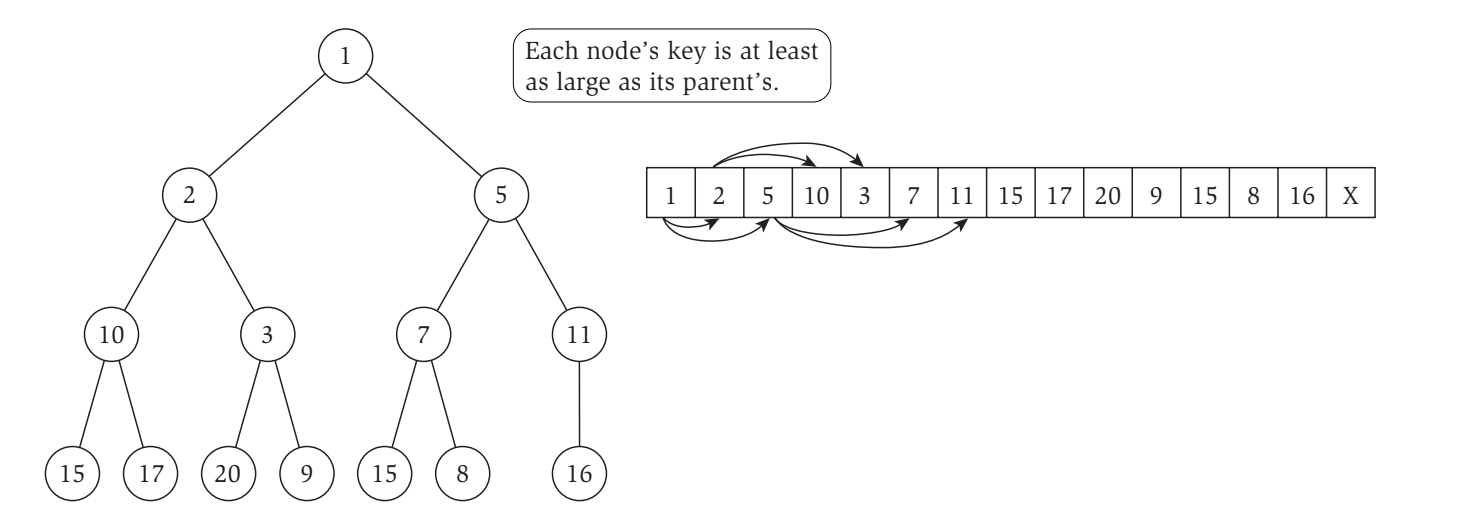
\includegraphics[width=0.7\textwidth ]{heap}
		\caption{An example of heap.}
\end{figure}

This data structure is very helpfull, instead of using an array or a list, here are the complexity of some operations involving the heap structure:

\[ create \; heap =  \mathcal{O}{(n)}\]
\[ insert \; heap =  \mathcal{O}{(logn)}\]
\[find \; min =  \mathcal{O}{(1)}\]
\[delete  =  \mathcal{O}{(logn)}\]

\end{itemize}

\clearpage

\section{Greedy Algorithms}

\emph{Formal definition}: the greedy algorithm "stays ahead" locally: meaning that is better than any other solutions, alternatively we can prove that a greedy algorithm's solution is optimal by transforming the know optimal solution for the problem, into our solution, this method is called "argument exchange".\\\\\emph{Practical definition}: A lot of the time a greedy algorithms involves scanning all the $n \in INPUT$ of the problem, if the current element respect some conditions, then it can be added to the optimal solution returned by the algorithm.

\subsection{The Cashier Problem / Coin changing}

Given a currency with the following values: 1, 5, 10, 25, 100, devise a method to pay amount to customer using fewest number of coins.\\\\
\emph{Example}: 34 dollars, how many coins?\\\\
\emph{Solution}: at each iteration, add coin of the largest value that does not take us past the amount to be paid.

\begin{algorithm}[H]
\SetAlgoLined
\small
\KwIn{$amount$ containing the amount to give back to the client, $C$ set containing all the coins of the current currency. }
\KwOut{$S$ the set containing all the coins to give back to the client}
\BlankLine


$S \leftarrow$ set containing all the coins to give back to the client\;
$total = 0 \leftarrow$ total expressed in the current currency system\;  
$Cs \leftarrow$ set containing all the coins in the currency sorted by increasing values\;

\BlankLine
\While{$total < amount $}{
	  \For{i=Cs.length to 0 }{
	  	\uIf{$total + Cs[i] < amount$}{
		$ total = total + Cs[i]$\;
         	$S = S \cup Cs[i]$\;
		$break;$
     		}
		\uElseIf{$total + Cs[i] = amount$}{
		$S = S \cup Cs[i]$\;
		$ return \; S$\;
     		}{}
	  }  
	  
}
\BlankLine

return $S$\;
\caption{cashierAlgorithm(amount,C):}
\end{algorithm}

\begin{claim}
The cashier algorithm always returns an optimal solution.
\end{claim}
\begin{proof}
The aim of the algorithm is to give as little change as possible (in terms of number of coins), if this is not true, then it must exist a solution $|S^{*}| < |S|$, but the algorithm always give highest compatible coin in the for loop, therefore a contradiction.
\end{proof}\
 
 \subsection{Interval Scheduling}
 
 We have a set J of jobs to execute on a machine and $\forall j \in J \; j=(s_{j},f_{j})$ where s and f are start and finish.Two jobs are compatible if the don't overlap: $\forall j_{i},j_{j} \in C \; f_{i} \geq s_{j} \; or \;vice-versa $.\\
Once we defined the problem, is just the matter of identifying the best strategy to sort all the jobs in J. Turns out, the best strategy is to sort all the jobs by finishing time, from first to last (for a former proof please check the professor's slide, but the main idea is to prioritize the jobs that release the machine as soon as possible).
 
\begin{algorithm}[H]
\SetAlgoLined
\small
\KwIn{$J$ set containing all the jobs}
\KwOut{$S$ the set containing all the compatible jobs}
\BlankLine

$S \leftarrow$ set containing all the compatible jobs\;
$Js \leftarrow$ set containing all the sorted jobs in increasing order of finishing time $f1 < .... f_{j}$

\BlankLine
\For{i=0 to Js.lenght }{
	  	\If{$J[i].start \geq S.last.finish$}{
			$S = S \cup Js[i]$
		}
		{}
	  }  

\BlankLine

return $S$\;
\caption{earliestFinishingTime(J):}
\end{algorithm}

\begin{claim}
The earliestFinishingTime always return an optimal solution.
\end{claim}
\begin{proof}
Assume this is not true, then it must exist a solution $|S^{*}| > |S|$,containing at least one more compatible job, but the algorithm check every job in J, therefore a contradiction.
\end{proof}\\

\begin{claim}
The complexity of the algorithm is $\mathcal{O}{(nlogn)}$
\end{claim}
\begin{proof}
The for loop costs $\mathcal{O}{(n)}$, while, as stated before, the sorting costs $\mathcal{O}{(nlogn)}$, since $\mathcal{O}{(nlogn)} > \mathcal{O}{(n)}$, the whole algorithm is $\mathcal{O}{(nlogn)}.$
\end{proof}\\

\subsection{Interval Partitioning}
Assuming we have a set of lectures L and, $\forall l \in L ,\; l=(s,f)$ where s and f are start time and finishing time, find the minimum amount of classroom tho schedule all the lectures, so that no two lectures overlap in the same classroom (the definition of overlap is the same as 3.2).

\begin{algorithm}[H]
\SetAlgoLined
\small
\KwIn{$L$ set containing all the lectures}
\KwOut{$S$ set containing the minimum amount of classroom needed}
\BlankLine

$S \leftarrow$ set containing the minimum amount of classroom needed\;
$Ls \leftarrow$ set containing all the sorted lectures in increasing order of starting time $s1 < .... s_{j}$

\BlankLine
\For{i=0 to Ls.lenght }{
	$C = \varnothing$
	
	\uIf{$J[i].start \geq C.last.finish$}{
    	$C = C \cup Ls[i]$\;
  	}
  	\Else{
   	 $S = S \cup C$\;
	 $C = \varnothing$\;
	$C = C \cup Ls[i]$\;
 	 } 
}  

\BlankLine

return $S$\;
\caption{intervalPartitioning(L):}
\end{algorithm}

The number of classrooms needed is more or equal to the depth of $|S|$, that is also the maximum amount of items that contains at any given time.	\\

\begin{claim}
The intervalPartitioning always return an optimal solution.
\end{claim}
\begin{proof}
Same as 3.2, if it exist a better solution $S^{*}$ we would have $|S^{*}| > |S|$ but that is not possible, since the algorithm checks every lecture in the input set. 
\end{proof}\\
 
\begin{claim}
The complexity of the algorithm is $\mathcal{O}{(nlogn)}$
\end{claim}
\begin{proof}
Identical as 3.2.
\end{proof}\\

\subsection{Minimizing The Lateness}
Assuming now we have just one resource that can process just one job at a time, we want to process all possible jobs. For the notation: $\forall j \in J,$ j requires  $t_{j}$ amount  of time to be executed, with a finishing time $f_{j} = s_{j} + t_{j}$, we have also to define a due date $d_{j}$ and finally the lateness of a job as: $max (0,d_{j}-f_{j})$

\begin{algorithm}[H]
\SetAlgoLined
\small
\KwIn{$L$ set containing all the lectures}
\KwOut{$S$ set containing the minimum amount of classroom needed}
\BlankLine

$S \leftarrow$ set containing all the compatible jobs\;
$Js \leftarrow$ set of all jobs sorted by increasing deadline $s1 < .... d_{j}$

\BlankLine
$t = 0 $\;
\For{i=0 to Js.lenght }{
	$s_{i} = t$\;
	$f_{i} = s_{i} + Js[i].finish$\;
	$S = S \cup (s_{i},f_{i})$\;
	$t = t + Js[i].time$\;
}  

\BlankLine

return $S$\;
\caption{earliestDeadLineFirst(J):}
\end{algorithm}

\begin{claim}
EarliestDeadLineFirst algorithm return an optimal solution.
\end{claim}
\begin{proof}
Identical as 3.2 / 3.3.
\end{proof}\\
 
\begin{claim}
The complexity of the algorithm is $\mathcal{O}{(nlogn)}$
\end{claim}
\begin{proof}
Identical as 3.2.
\end{proof}\\

\clearpage

\subsection{Dikstra Algorithm}

\emph{Def}: A path is a sequence of edges which connects a sequence of nodes.\\\\
\emph{Def}: A cycle is a path with no repeated nodes or edges other than the
starting and ending nodes.\\\\
\emph{Shortest Path problem}: Given a digraph G = (V, E), edge lengths $le \geq 0$, source $s \in V$, and destination $t \in V$, find the shortest directed path from s to t.

\begin{figure}[H]
		\centering
		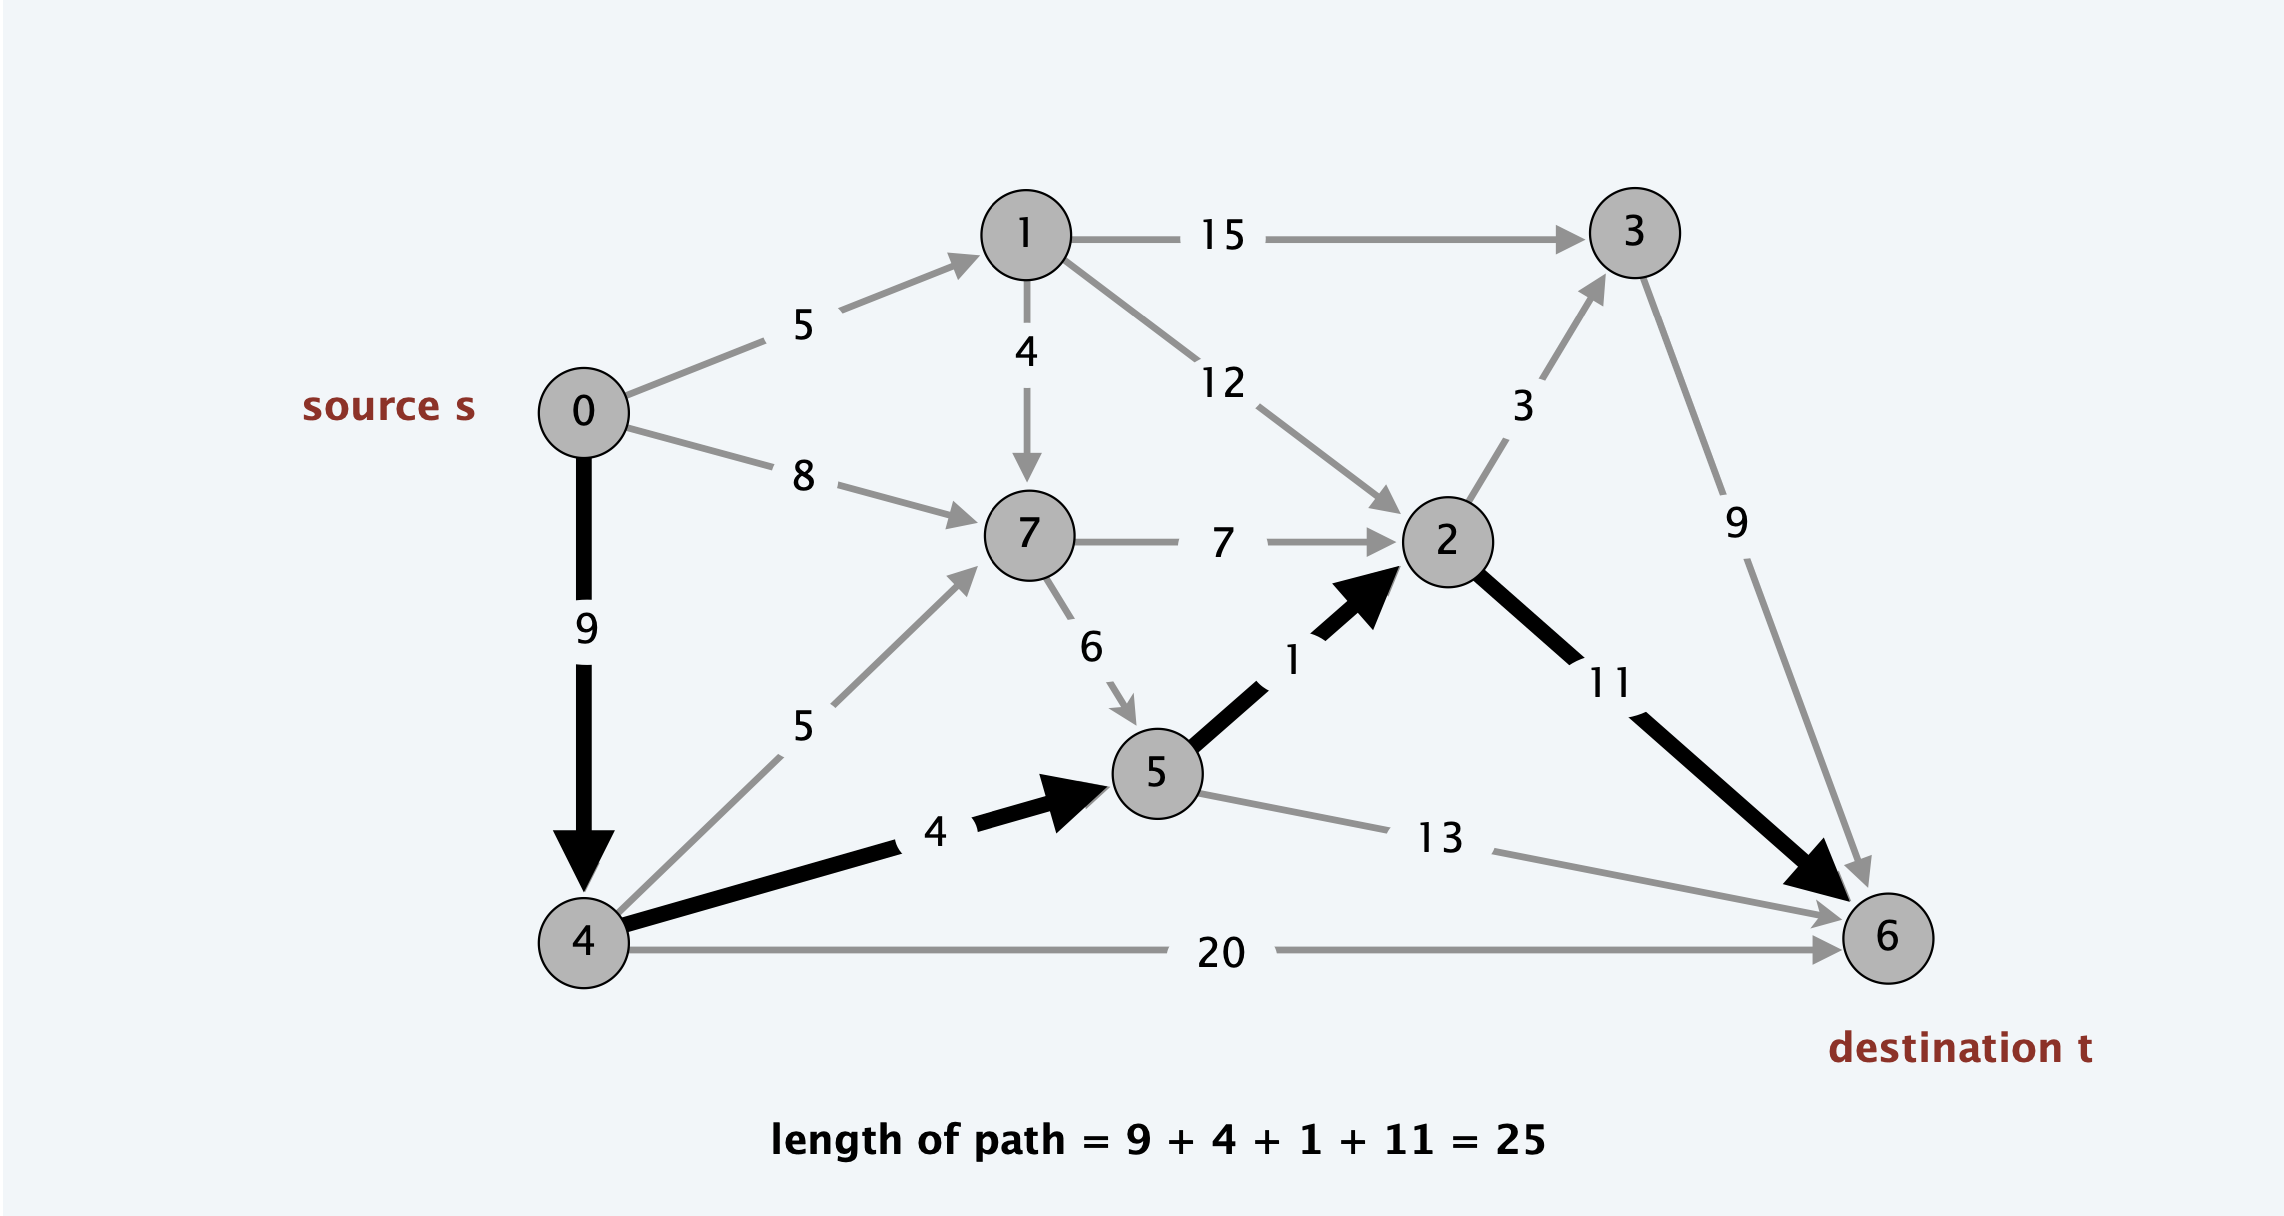
\includegraphics[width=0.8\textwidth ]{dikstra}
		\caption{A solution for the Shortest path problem.}
\end{figure}

\begin{algorithm}[H]
\SetAlgoLined
\small
\KwIn{$G$ set containing all the edges of G, $s$ source of the path}
\KwOut{$S$ set containing all the edges of a shortest path}
\BlankLine

$S \leftarrow$ set containing all the compatible jobs\;
$Q \leftarrow$ priority queue for nodes contained in the unexplored part of G \;
$D \leftarrow$ set of distances from s $\forall \; e \in G$

\BlankLine

$d(s,s) = 0$\;
$D = D \cup d(s,s))$\;

\BlankLine

\For{i=0 to G.lenght }{
	$e_{i} = G[i] \leftarrow$ current edge to check\;
	\uIf{$e_{i} \neq s$}{
	$d(s,e_{i}) = \infty$\;
    	$D = D \cup d(s,e_{i}))$\;
	$Q = Q \cup (e_{i},d(s,e_{i})) \leftarrow$ Insert in queue the current node with key($e_{i}$) = $d(s,e_{i})$\;
  	}
}

\BlankLine

\While{$Q \neq  \emptyset$}{
$u = Q.getMin $\;
$Q = Q - \{u\} $\;
\ForEach {$(u,v) \in G, \; leaving \; u $}{
\uIf{$d(s,v) > d(s,u) + l(u,v)$}{
	$S = S \cup  d(s,u) + l(u,v) $\;
	decrease-key of v to d(u) + l(u, v) in Q.\;
}	
}
}

return $S$\;
\caption{Dikstra(G,s):}
\end{algorithm}

\begin{claim}
The Dikstra Algorithm always return an optimal solution ($\forall u \in S, \; d(u)$ is the length of the shortest $s\rightarrow u$ path).
\end{claim}
\begin{proof}
Base case: $| S |$ = 1 is easy since S = { s } and d(s) = 0, assume that's true for $| S | > 1$:\\
let t be next node added to S, and let (u, t) be the final edge: the shortest $s\rightarrow u$ path + (u, t) = $s\rightarrow t$ path of length $π(t)$.\\\\Now consider any $s\rightarrow t$ path P: it's is no shorter than $π(t)$. Let (x, y) be the first edge in P that leaves S, and let P' be the subpath to x, P is already too long as soon as it reaches y, so putting all together:
\[l( P ) \geq l( P ' ) + l( x , y ) \geq d ( x ) + l( x , y ) \geq π ( y ) \geq π (t)\]
\end{proof}\\

\begin{claim}
The Dikstra Algorithm complexity, for a graph G=(V,E), using a priority queue is: $\mathcal{O}{((V + E) \; log\; V)}$.
\end{claim}

\begin{proof}
It highly depends on the type of queue used, but we have to check all the nodes in the priority queue plus all the edges coming out of every node, for further detail, please check the professor's slides.
\end{proof}\\


\subsection{Kruskal Algorithm}
Given an undirected, weighted, connected graph G=(V,E) we want to find the all the edges that connects all the nodes with a minimum cost, alternatively we can say that the algorithm finds the minimum spanning tree (MST) of G.\\\\
\emph{Formal definition}: Given an undirected, weighted, connected  graph G = (V, E) with edge costs $c(e)$, an MST is a subset of the edges $T \subseteq E$ such that T is a spanning tree whose sum of edge costs is minimized.

\begin{figure}[H]
		\centering
		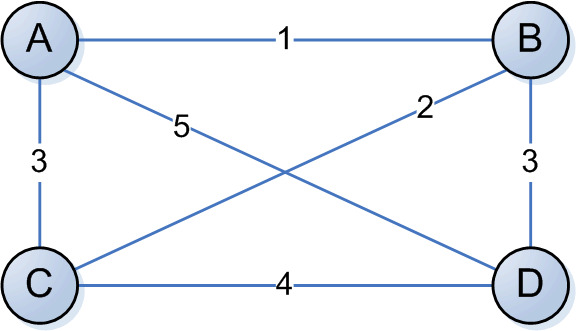
\includegraphics[width=0.4\textwidth ]{kruskal}
		\caption{An instance of the MST problem.}
\end{figure}

\begin{figure}[H]
		\centering
		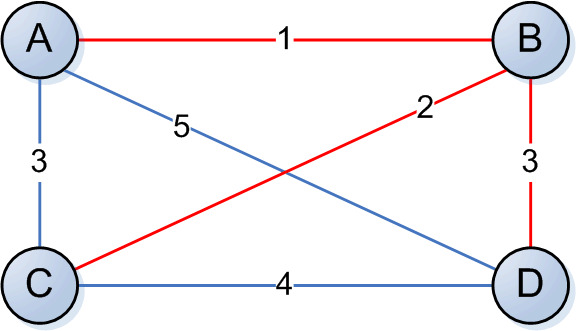
\includegraphics[width=0.4\textwidth ]{kruskal_solved}
		\caption{A solution for the MST problem.}
\end{figure}

\begin{algorithm}[H]
\SetAlgoLined
\small
\KwIn{$G$ set containing all the edges of G}
\KwOut{$S$ set containing all the edges of MST}
\BlankLine

$S \leftarrow$ set containing all the compatible jobs\;
$E \leftarrow$ set of all the edges sorted by increasing weight $c(e)_{1} < .... c(e)_{j}$

\BlankLine

\For{i=0 to G.lenght }{
	$e_{i} = G[i] \leftarrow$ current edge to check\;
	\uIf{$S \cup e_{i} \;is \;not \;a \;loop$}{
    	$S = S \cup e_{i}$ \;
  	}
}  

\BlankLine

return $S$\;
\caption{kruskal(G):}
\end{algorithm}

\begin{claim}
Kruskal algorithm returns an optimal solution.
\end{claim}
\begin{proof}
Identical as 3.2 / 3.3.
\end{proof}\\
 
\begin{claim}
The complexity of the algorithm is $\mathcal{O}{(nlogn)}$
\end{claim}
\begin{proof}
Identical as 3.2.
\end{proof}\\

\clearpage
\section{Dynamic Programming}

\emph{Formal definition}: Break up a problem into a series of overlapping subproblems, and build up solutions to larger and larger subproblems.\\\\\emph{Practical definition}: A lot of the times dynamic programming involves taking the best possible result of the subproblem (that maximizes the overall results), and store it in a data structure so it should not be recomputed later: this process is called memoization.For an algorithm dealing with dynamic programming usually there are 2 possible approaches:\\

\begin{itemize}

\item {Top-down}\\\\
The most common approach: as we said we divide the problem, into sub-problems and recursively memorize the result in a table (again using the memoization tecnique), whenever attempting to solve the sub-problems, we first check if we already computed the result in the table, saving precious execution time.

\item {Bottom-up}\\\\
We formulate the solution to a problem recursively by solving the subproblems first, and then using their solutions to formulate a larger overall solution.

\end{itemize}

\subsection{Weighted Interval Scheduling}

Same as 3.2 but this time $\forall j \in J$, there is an associated weight $w(j) > 0$, in this case, unfortunately, the greedy algorithm fails.\\
To find a possible solution, we start to label jobs by finishing time $f1 \leq f2 \leq . . . \leq f_{n}$ and we donote with $p_{j}$ = the largest index $i < j$ such that job i is compatible with j:

\begin{figure}[H]
		\centering
		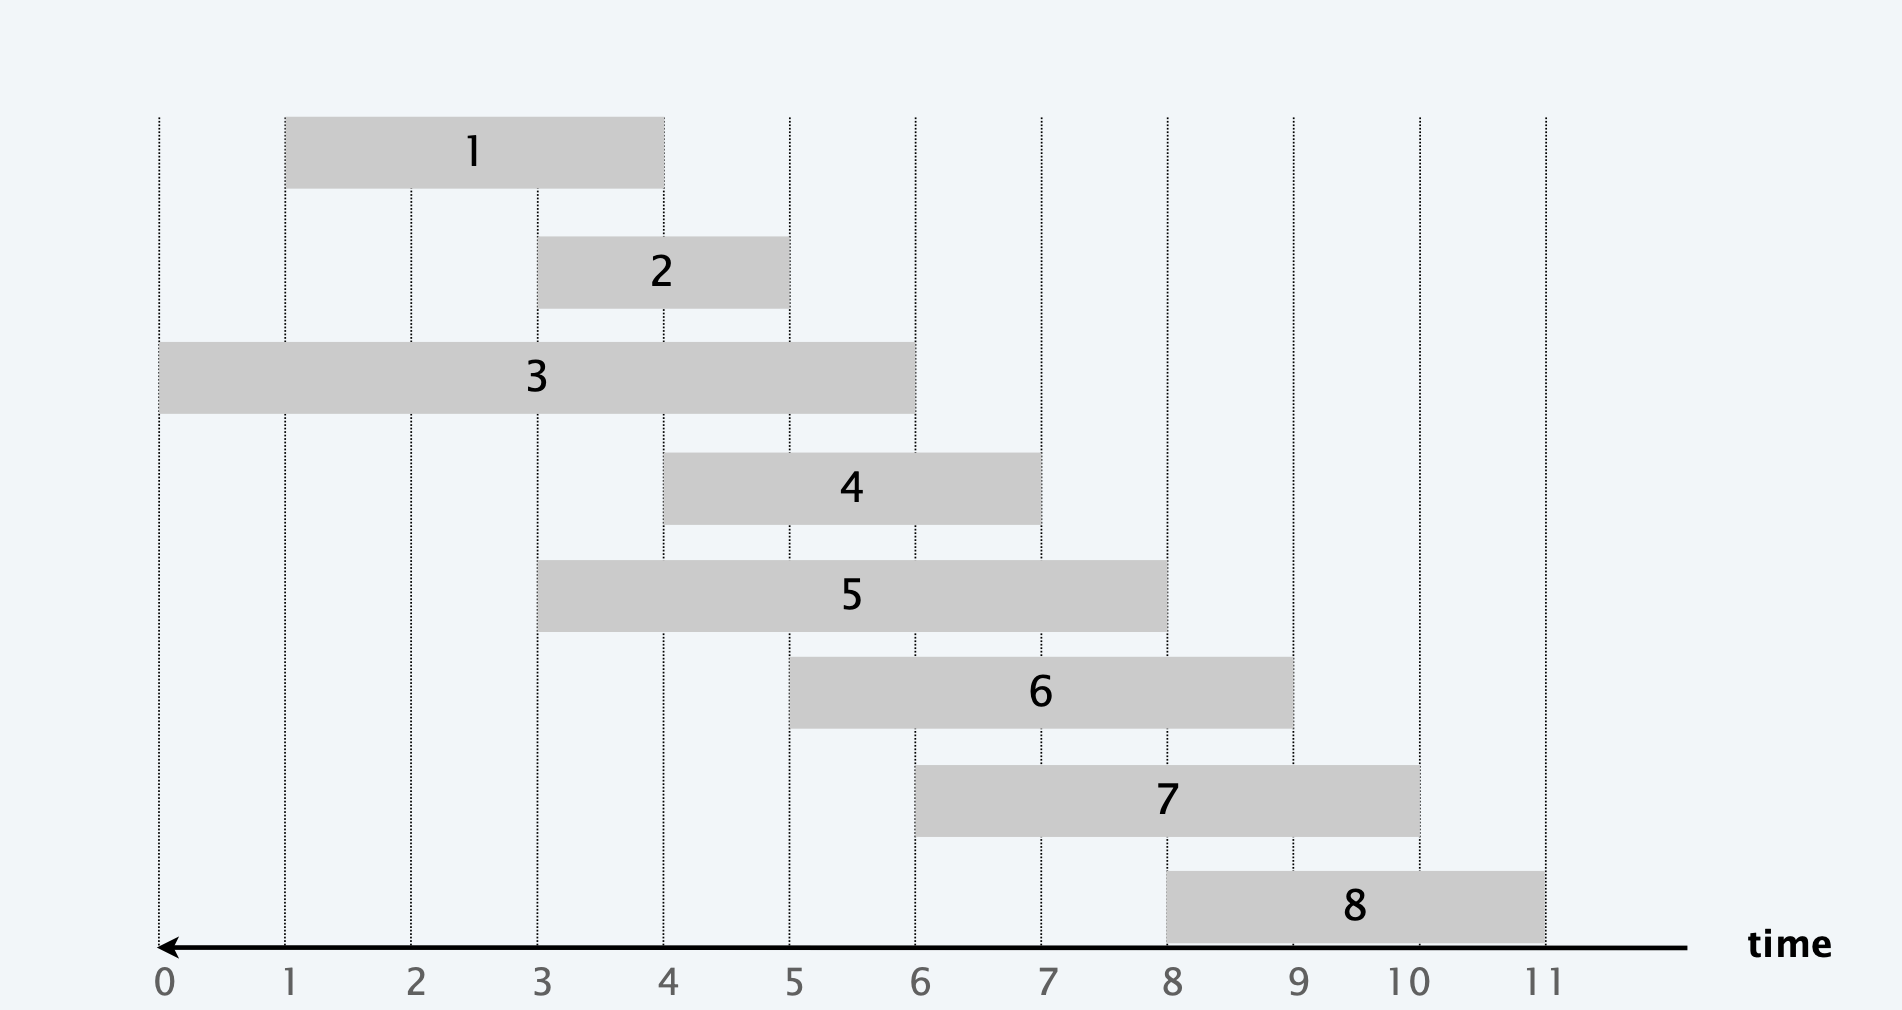
\includegraphics[width=0.7\textwidth ]{weighted}
		\caption{An instance for the weighted scheduling problem.}
\end{figure}

Example p(8) = 5 because the earliest compatible $j \in J$ with $j_{8}$ is $j_{5}$.More examples: p(7) = 3, p(2) = 0, ecc...\\\\
Now let's denote the OPT(j) as the value of optimal solution to the problem consisting, of job requests $1, 2, ..., j$. When dealing with dynamic programming, we have to build a formal definition of the recursion function, that defines the optimum at every step, but first we have to understand what happen at each iteration of the algorithm, the optimum can either:

\begin{itemize}

\item {OPT selects job j}\\\\
The algorithm then collect the profit $v_{j}$, then is locked out by all the incompatible jobs $\{ p(j) + 1, p(j) + 2, ..., j – 1 \}$, but must contain all the remain compatible jobs $\{1, 2, ..., p(j)\}$.

\item {OPT does not select job j}\\\\
Must include optimal solution to problem consisting of remaining compatible jobs $\{1, 2, ..., j – 1\}$.

Merging all these informations we can build the recursion function:

\[OPT(j) = \begin{cases} 0 \; if \; j = 0 \\ max\{vj \; + \; OPT(p(j)), OPT(j−1)\}  \end{cases}\]

\end{itemize}

Now for the implementation:

\begin{algorithm}[H]
\SetAlgoLined
\small
\KwIn{$J$ set of jobs, each one with a $s_{j}$ start time, a finishing time $f_{j}$ and a reward $v_{j}$}
\KwOut{$S$ containing the largest amount of compatible weighted jobs}
\BlankLine

$Js \leftarrow$ all the jobs sorted by increasing finishing time $f_{1} \leq f_{2} ... f_{j}$

\BlankLine

\For{i=0 to J.lenght }{
	\uIf{$i = 0$}{
    	$M[i] = 0$ \;
  	}
	\uElse{
	$M[i] = \emptyset$ \;

	}
}

\BlankLine

$costMatrix = MComputeOpt(M,Js,J.last)$\;
$return findSolution(M,currentJob)$

\caption{DynamicWeightedInterval(J):}
\end{algorithm}

\begin{algorithm}[H]
\SetAlgoLined
\small
\KwIn{$M$ Initialized Matrix containing all the reward,\; $J$ set of jobs, $currentJob$ to calculate the reward.}
\KwOut{$M$ matrix containing all the computed values for each job}

\BlankLine
	
	\uIf{$M[currentJob] = \emptyset$}{
    	$M[currentJob] = max(currentJob.vj  + MComputeOpt(M,J,currentJob.pj), MComputeOpt(M,J,J[currentJob – 1]))$ \;
  	}
	\uElse{
	$return \; M[currentJob]$ \;
	}

\BlankLine

\caption{MComputeOpt(M,J,currentJob):}
\end{algorithm}

\begin{algorithm}[H]
\SetAlgoLined
\small
\KwIn{$M$ Initialized Matrix containing all the reward,\; $currentJob$ to calculate the reward.}
\KwOut{$S$  containing the largest amount of compatible weighted jobs}
\BlankLine

	\uIf{$currentJob = 0$}{
    	return $\emptyset$ \; 	
	}
	\uElseIf{$currentJob.v_{j} + M[currentJob.p_{j}] > M[currentJob–1]$}{
	$return \{ j \} \cup FindSolution(M,currentJob.p_{j}).$
	}
	\uElse{
	$FindSolution(M,currentJob-1).$
	}

\BlankLine

\caption{findSolution(M,currentJob):}
\end{algorithm}

\begin{claim}
The algorithm runs in $\mathcal{O}{(nlogn)}$
\end{claim}

\begin{proof}
The recursive processes takes $\mathcal{O}{(n)}$ each, the most computational intensive operation is the sorting that takes $\mathcal{O}{(nlogn)}$, so overall we have $\mathcal{O}{(2n + nlogn)} \simeq$ $\mathcal{O}{(nlogn)} .$  
\end{proof}

\subsection{Knapsack Problem}
Given N objects and a Knapsack(it's a backpack) with a capacity W, we have $\forall n \in N, \; w_{n} \geq 0 \; v_{n} \geq 0$, the goal is to fillup the Knapsack without exceeding it's capacity with the maximum value.

\begin{figure}[H]
		\centering
		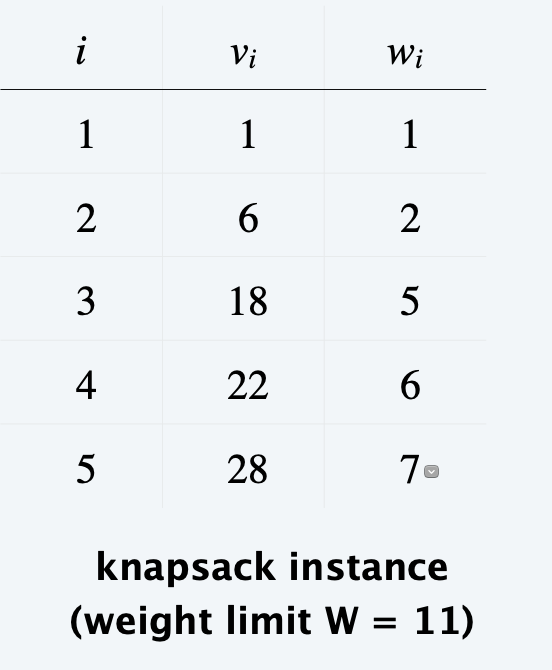
\includegraphics[width=0.2\textwidth ]{knapsack}
		\caption{An instance for the knapsack problem.}
\end{figure}

Example: $\{ 1, 2, 5 \}$ has value 35,  $\{ 3, 4 \}$ has value 40, $\{ 3, 5 \}$ has value 46 (but exceeds weight limit).

\begin{itemize}

\item {Defining the Optimum}\\

This time we have to take into account both the variation of the value of the content of the knapsack and the weight limit left:

\[OPT(j) = \begin{cases} 0 \; if \; i = 0 \\ OPT(i-1,w) \; if \; w_{i} > w \\ max\{OPT(i−1,w),\; vi + OPT(i−1,w−w_{i})\} \; otherwise \}  \end{cases}\]

\end{itemize}

Now for the implementation:

\begin{algorithm}[H]
\SetAlgoLined
\small
\KwIn{$N$ set of all the objects, each one with a $v_{j}$ value, and $w_{i}$ weight, $W$ the maximum capacity of the knapsack}
\KwOut{$S$ containing the most valuable objects without exceeding w}
\BlankLine

\BlankLine

\For{i=0 to w }{
	$M[0,wi] = 0$ \;
}
\For{j=1 to $N$ }{
\For{k=1 to $W$ }{
	\uIf{$N[j].weight > k$}{
    	$M[j,k] = M[j–1,k]$	
	}
	\uElse{
	$M [ j, k ] =  max \{ M [ j – 1, k], vi + M [ j – 1, w – w_{j}] \}$.
	}	
}
}


\BlankLine
return $M[n,W]$

\caption{DynamicKnapsack(N,W):}
\end{algorithm}

\begin{figure}[H]
		\centering
		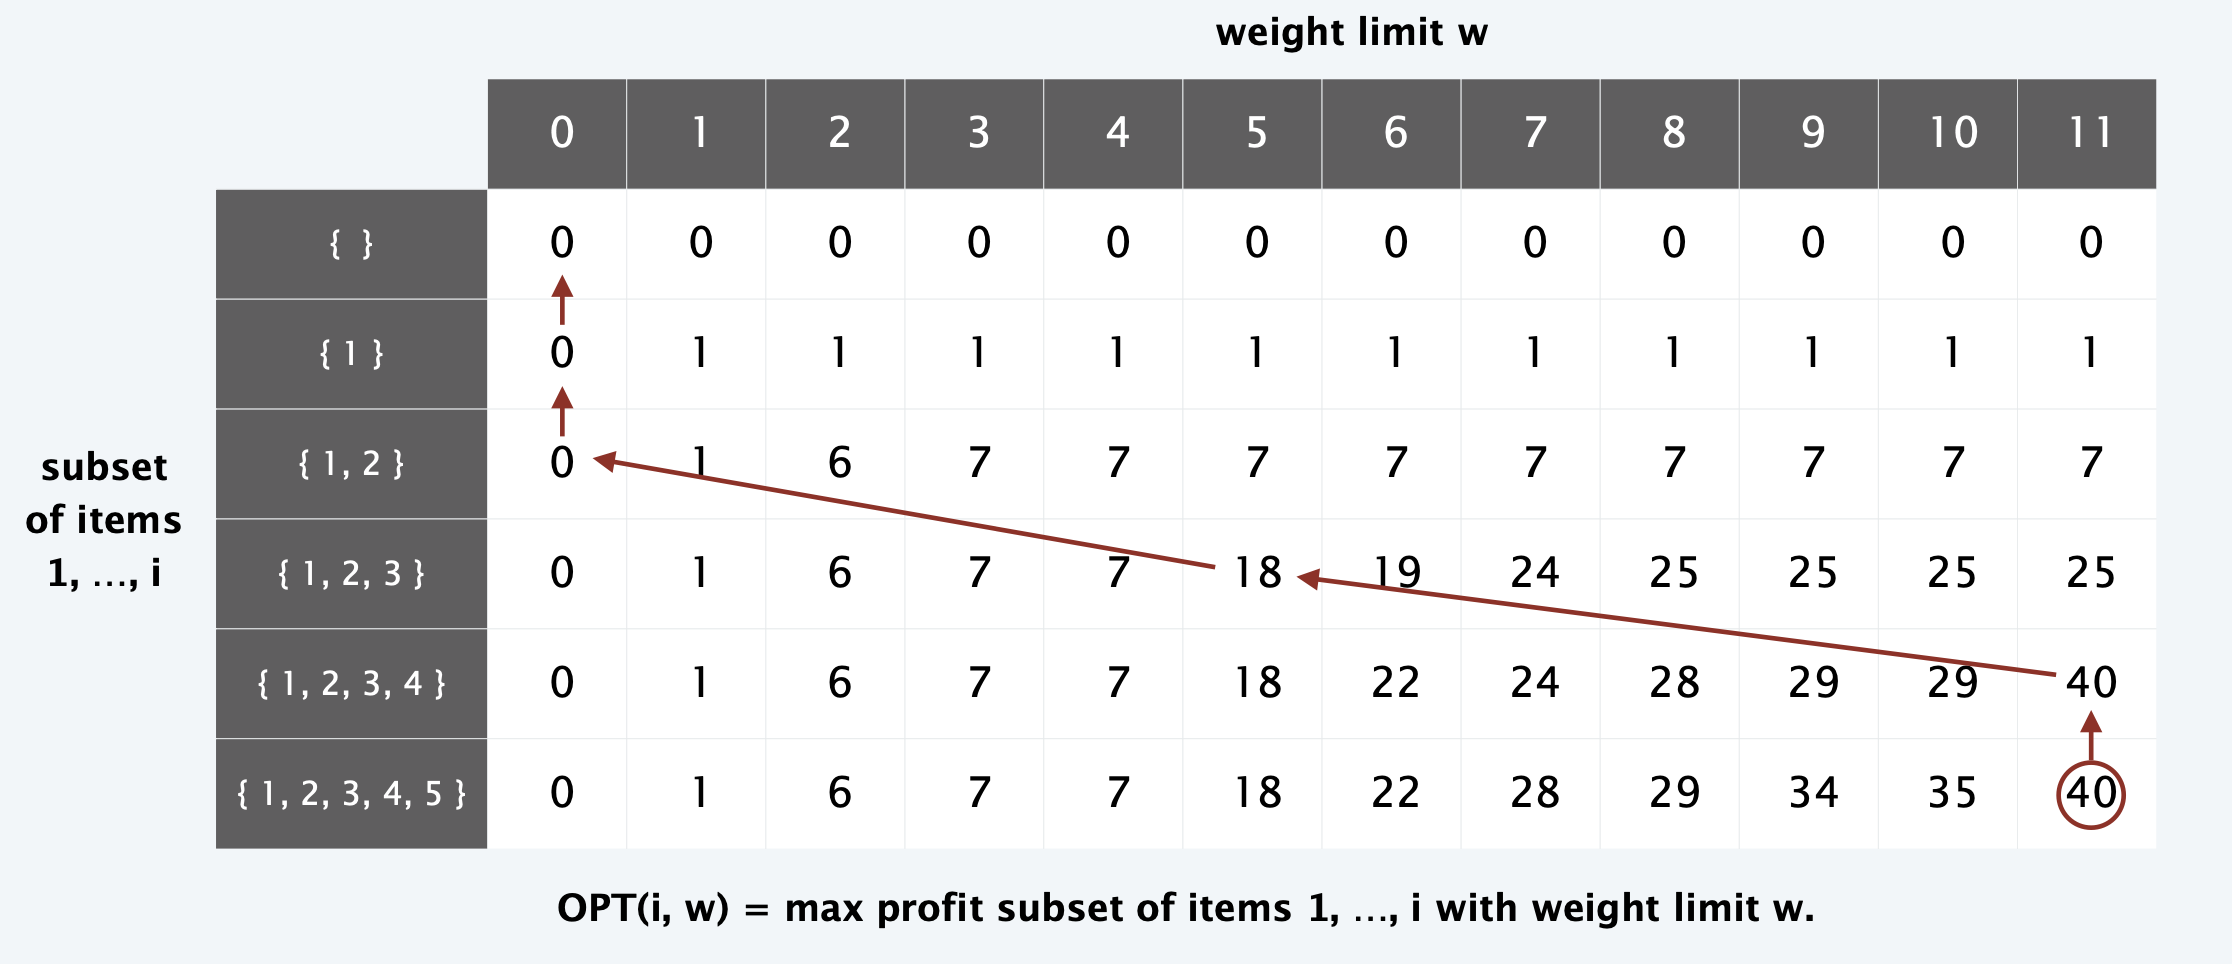
\includegraphics[width=0.8\textwidth ]{knapsack2}
		\caption{A table rapresenting the solution for the knapsack problem.}
\end{figure}

This algorithm is defined as pseudo-polinomial, because the execution time is proportional to the knapsack's W.\\

\begin{claim}
The algorithm runs in Θ(nW)
\end{claim}

\begin{proof}
We need to build a table of all the combinations of values and weight of dimension Θ(nW), $\forall n \in N$ so that's the execution time of the algorithm.
\end{proof}

\subsection{Sequence Alignment}
In this problem we want to measure the degree of similarity between two strings, first of all we have to make sure that the two strings have the same length, then we define a gap as $ \exists i \in s_{1} / s_2[i] = \emptyset$ or vice-versa, instead a mismatch as: $\exists i \in s_{1} / s_2[i] \neq s_{1}[i]$.

\begin{figure}[H]
		\centering
		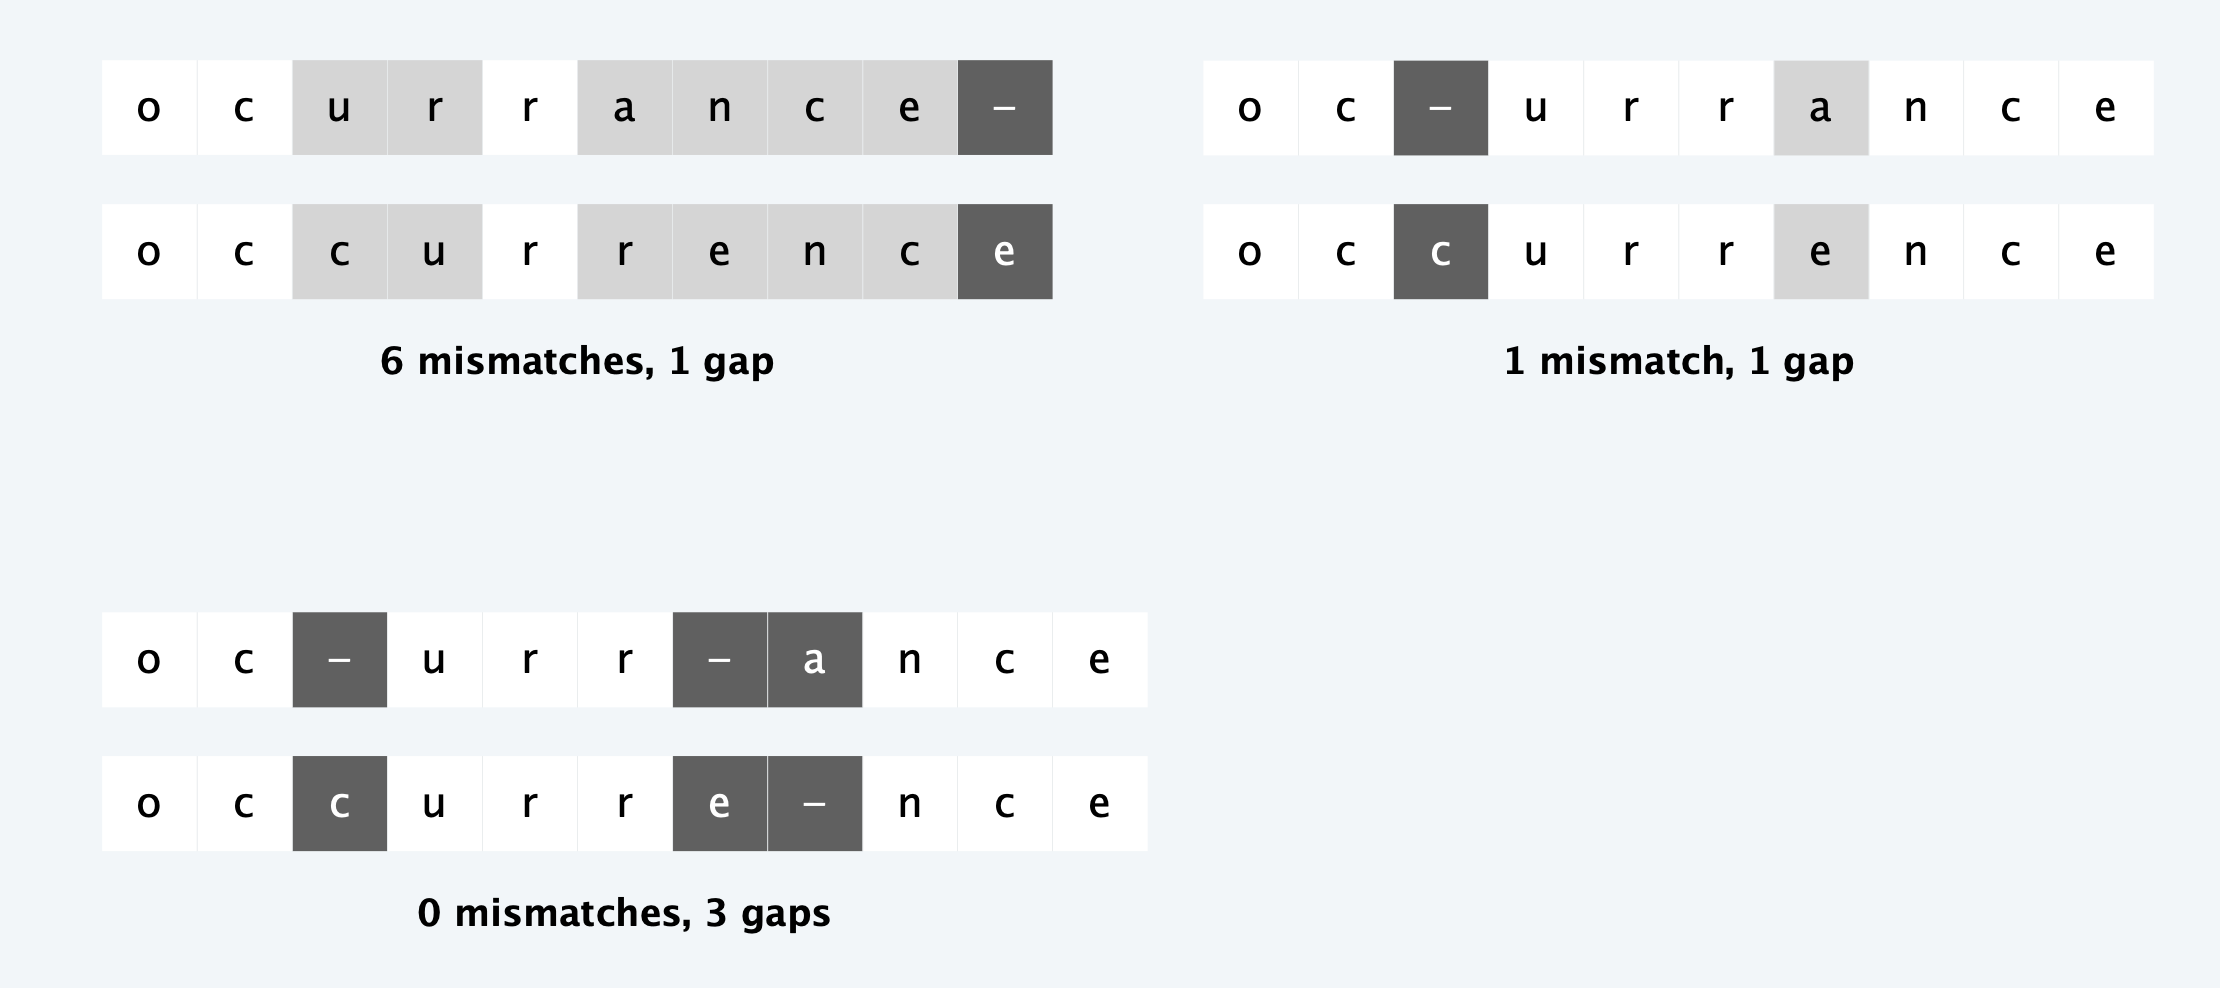
\includegraphics[width=0.6\textwidth ]{sequence}
		\caption{different approaches for the gap and occurrences in the sequence alignment problem.}
\end{figure}

To define a degree of similarities between two strings, we need a way to define a cost that rappresents the degree of difference between the strings, so for each gap we define a penalty $\delta$ and a mismatch penalty $\alpha_{p,q}$, so the total cost would be the sum of mismatch and gaps. Now we can re-formulate our problem as: given two strings $x_{1},x_{2}...x_{m}$ and $y_{1},y_{2}...y_{m}$, we want to find a minimum cost alignment defined as: a set of ordered pairs $x_{i} - y_{i}$ such that each item occurs in at most one pair and no crossings ($x_{i} – y_{j}$ and $x_{i'} – y_{j'}$ cross if $i < i '$, but $j > j '$).

\begin{figure}[H]
		\centering
		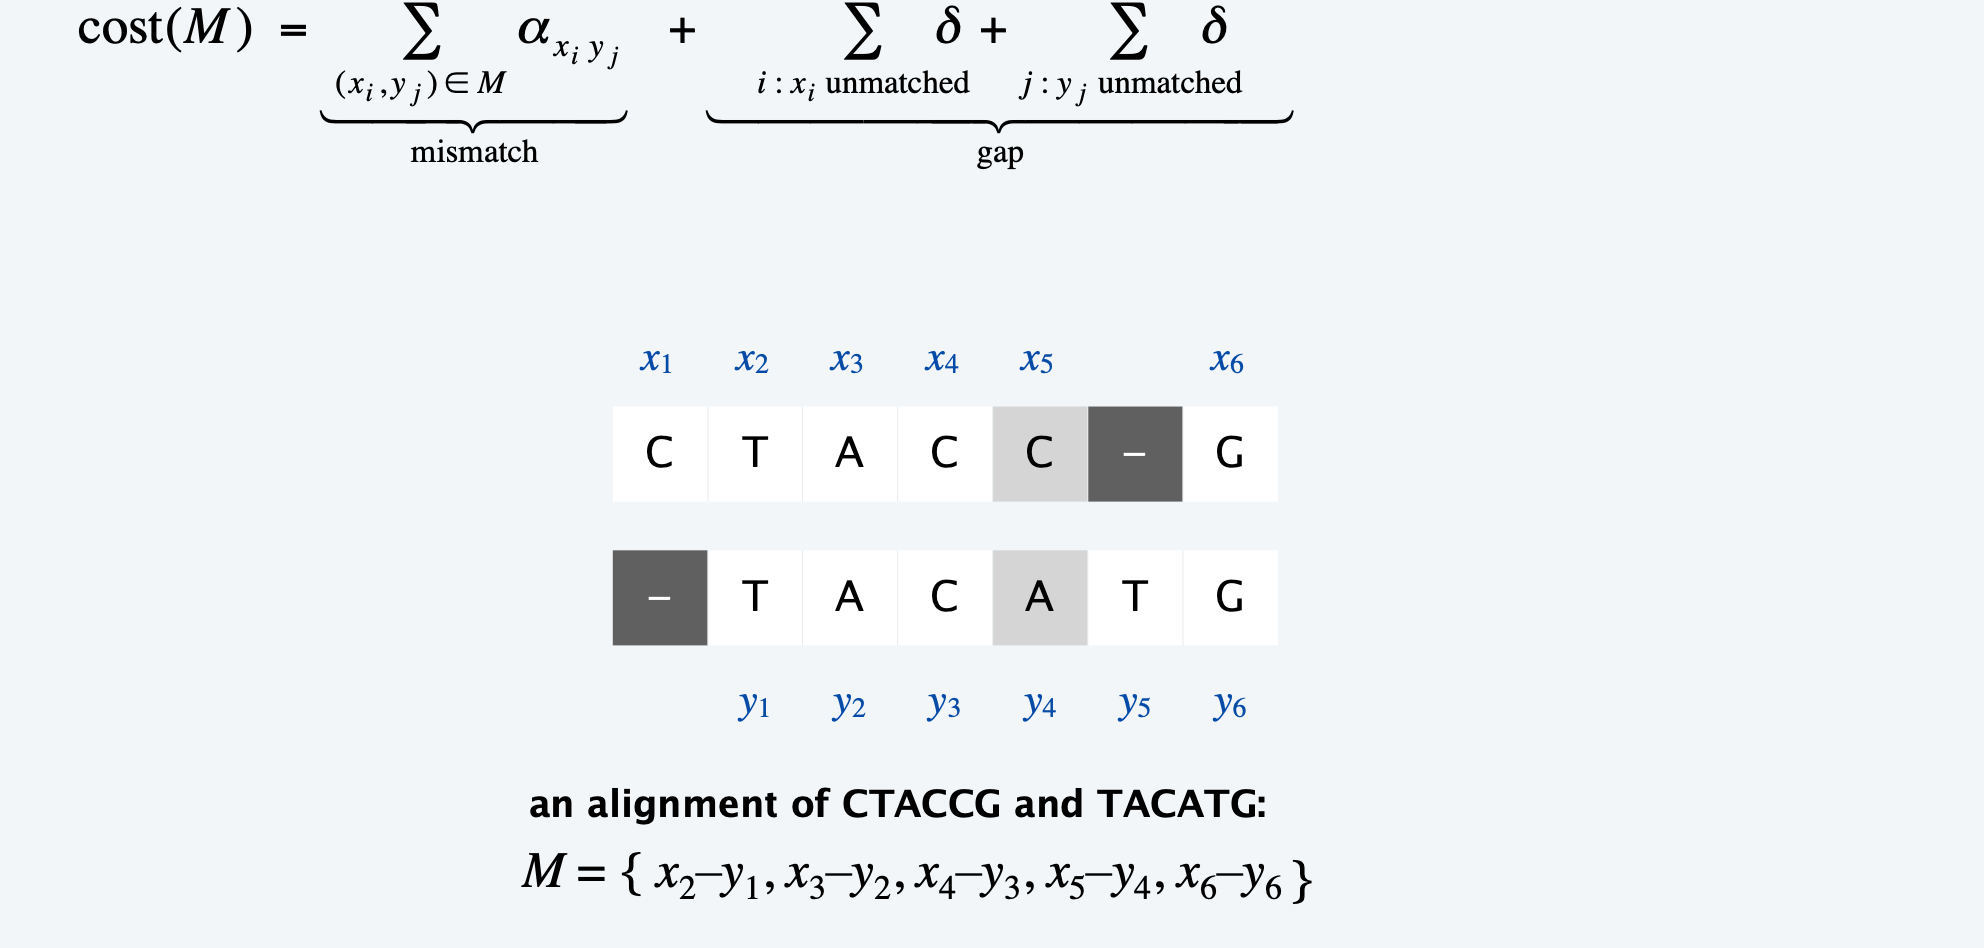
\includegraphics[width=0.6\textwidth ]{sequence2}
		\caption{Cost Definition.}
\end{figure}

Now, as usual we have to define the optimum as OPT(i, j) = min cost of aligning prefix in the two strings.

\begin{itemize}

\item {Case 1: matches $x_{i} – y_{j}$.}\\
Pay mismatch for $x_{i} – y_{j}$ + min cost of aligning $x_{1}, x_{2} ... x_{i–1}$ and $y_{1} ,y_{2} ... y_{j–1}$.

\item {Case 2:OPT leaves $x_{i}$ unmatched.}\\
Pay gap for $x_{i}$ + min cost of aligning $x_{1}, x_{2} ... x_{i–1}$ and $y_{1}, y_{2} ... y_{j}$.

\item {Case 3:OPT leaves $y_{i}$ unmatched}\\
Pay gap for $y_{j}$ + min cost of aligning $x{_1},x_{2} ... x{i}$ and $y_{1}, y_{2} ... y_{j}$.

\end{itemize}

\[OPT(j) = \begin{cases} i\delta \; if \; i = 0 \\ min \;otherwise \\ j\delta \; j=0 \}  \end{cases}\]
\[min=\begin{cases} \alpha _{x_{i} y_{j}} OPT(i−1, j-1) \\ \delta OPT(i−1, j) \\ \delta  O P T ( i , j − 1 )  \end{cases}\]


\begin{algorithm}[H]
\SetAlgoLined
\small
\KwIn{$x$ String $y$ String}
\KwOut{$S$ containing the minimum cost alignment.}

\BlankLine

\For{i=0 to x.lenght }{
	$M[i,0] = \delta i$ \;
}

\BlankLine

\For{j=0 to y.lenght }{
	$M[j,0] = \delta j$ \;
}

\BlankLine

\For{i=0 to x.lenght }{
	\For{j=0 to y.lenght }{
	$M[i,j] = min(\alpha[x_{i}, y_{j}] + M[i–1, j–1], \delta + M[i–1, j],\delta + M[i, j–1]) $\;
}
}

\BlankLine
return S = M[x.lenght][y.lenght]


\caption{SequenceAllignment(x,y):}
\end{algorithm}

\begin{claim}
The algorithm runs in Θ(mn) for two strings of length m and n.
\end{claim}

\begin{proof}
We need to build a table of all the combinations of values and weight of dimension Θ(mn), same as 4.2
\end{proof}

\subsection{Bellman-Ford}
Algorithm for shortest path for graphs with negatives paths, unfortunately the Dikstra fails:

\begin{figure}[H]
		\centering
		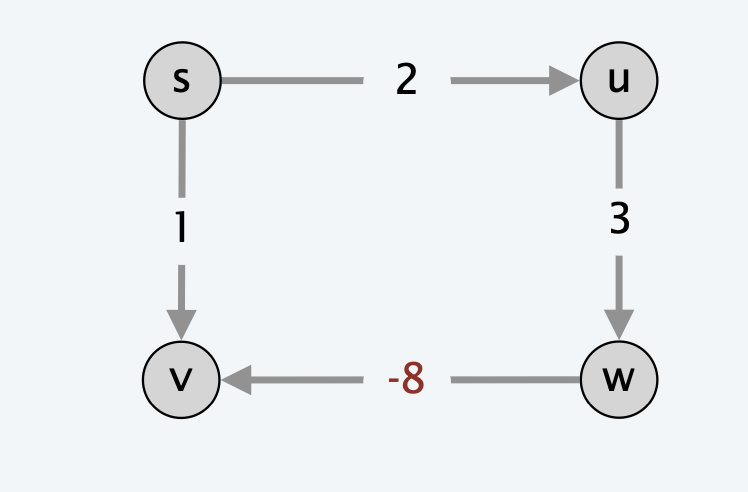
\includegraphics[width=0.3\textwidth ]{bellman}
		\caption{G=(V,E) with negative paths: the Dikstra algorithm will select c(s,v) = 1, ignoring the correct solution: c((s,u)+(u,w)+(w,v))=-3}
\end{figure}

\emph{Formal definition}:A negative path is a directed cycle such that the sum of its edge weights is negative.
\[ c(W) = \sum_{e \in W}^{} c_{e} < 0 \]

\begin{claim}
If some path from v to t contains a negative cycle, then there does not exist a cheapest path from v to t.
\end{claim}\\

\begin{proof}
If there exists such a cycle W, then can build a $v \rightarrow t$ path of arbitrarily negative weight by detouring around cycle as many times as desired.
\end{proof}\\

\begin{claim}
If G has no negative cycles, then there exists a cheapest path from v to t that is simple (and has $\leq$ n – 1 edges).
\end{claim}

\begin{proof}
Consider a cheapest $v\rightarrow t$ path P that uses the fewest number of edges, If P contains a cycle W, we can remove portion of P corresponding to W
without increasing the cost.
\end{proof}\\

the OPT(i,v) = cost of shortest $v\rightarrow t$ path that uses i edges, with i $\leq |E|$.

\begin{itemize}

\item {Case 1: Cheapest  $v\rightarrow t$ path uses $\leq$ i – 1 edges.}\\
OPT(i, v) = OPT(i – 1, v)

\item {Case 2:Cheapest  $v\rightarrow t$ path uses $\leq$ i edges.}\\
if (v, w) is first edge, then OPT uses (v, w), and then selects best $w \rightarrow t$ path using $\leq$ i – 1 edges.


\end{itemize}

\[OPT(i,v) = \begin{cases} \infty \; if = 0  \\ min \; otherwise \end{cases}\]
\[min= \{ OPT(i-1,v),min_{(v,w) \in E} \{OPT(i−1, w)+c_{vw} \}\} \]

Implementation:

\begin{algorithm}[H]
\SetAlgoLined
\small
\KwIn{$G$ directed graph with negative paths\; $s$ source node of the path, $t$ final node of the path.}
\KwOut{$S$ containing the shortest path s $\leftarrow$ t}

\BlankLine
	

\BlankLine

\caption{BellmanFord(G,s,t):}
\end{algorithm}

\begin{claim}
The Bellman-Ford algorithm's cost is $\mathcal{O}{(nm)}$.
\end{claim}
\begin{proof}
The successor graph cannot have a negative cycle,thus, following the successor pointers from s yields a directed path to t.\\
Let $s = v_{1} \leftarrow v_{2} \leftarrow ... \leftarrow v_{k} = t$ be the nodes along this path P, upon termination, if successor(v) = w, we must have d(v) = d(w) + $c_{vw}$, putting it all together, we have:
	\[d(s) = d(t) + c(v_{1}, v_{2}) + c(v_{2}, v_{3}) + ... + c(v_{k–1}, v_{k})\]
\end{proof}


\clearpage

\section{Network Flow}
A flow network is a grap G=(V,E) with source $s \in V$ and $t \in V$, with $\forall e \in E, \; c(e) \geq 0$.An $s \rightarrow t$ cut is a partition (A, B) of the vertices with $s \in A$ and $ t \in B$, while the capacity is the sum of all the capacities of all the edges from A to B: cap(A,B) = $ \sum_{e \; out \; of \; A}^{} c_{e}$

\begin{figure}[H]
		\centering
		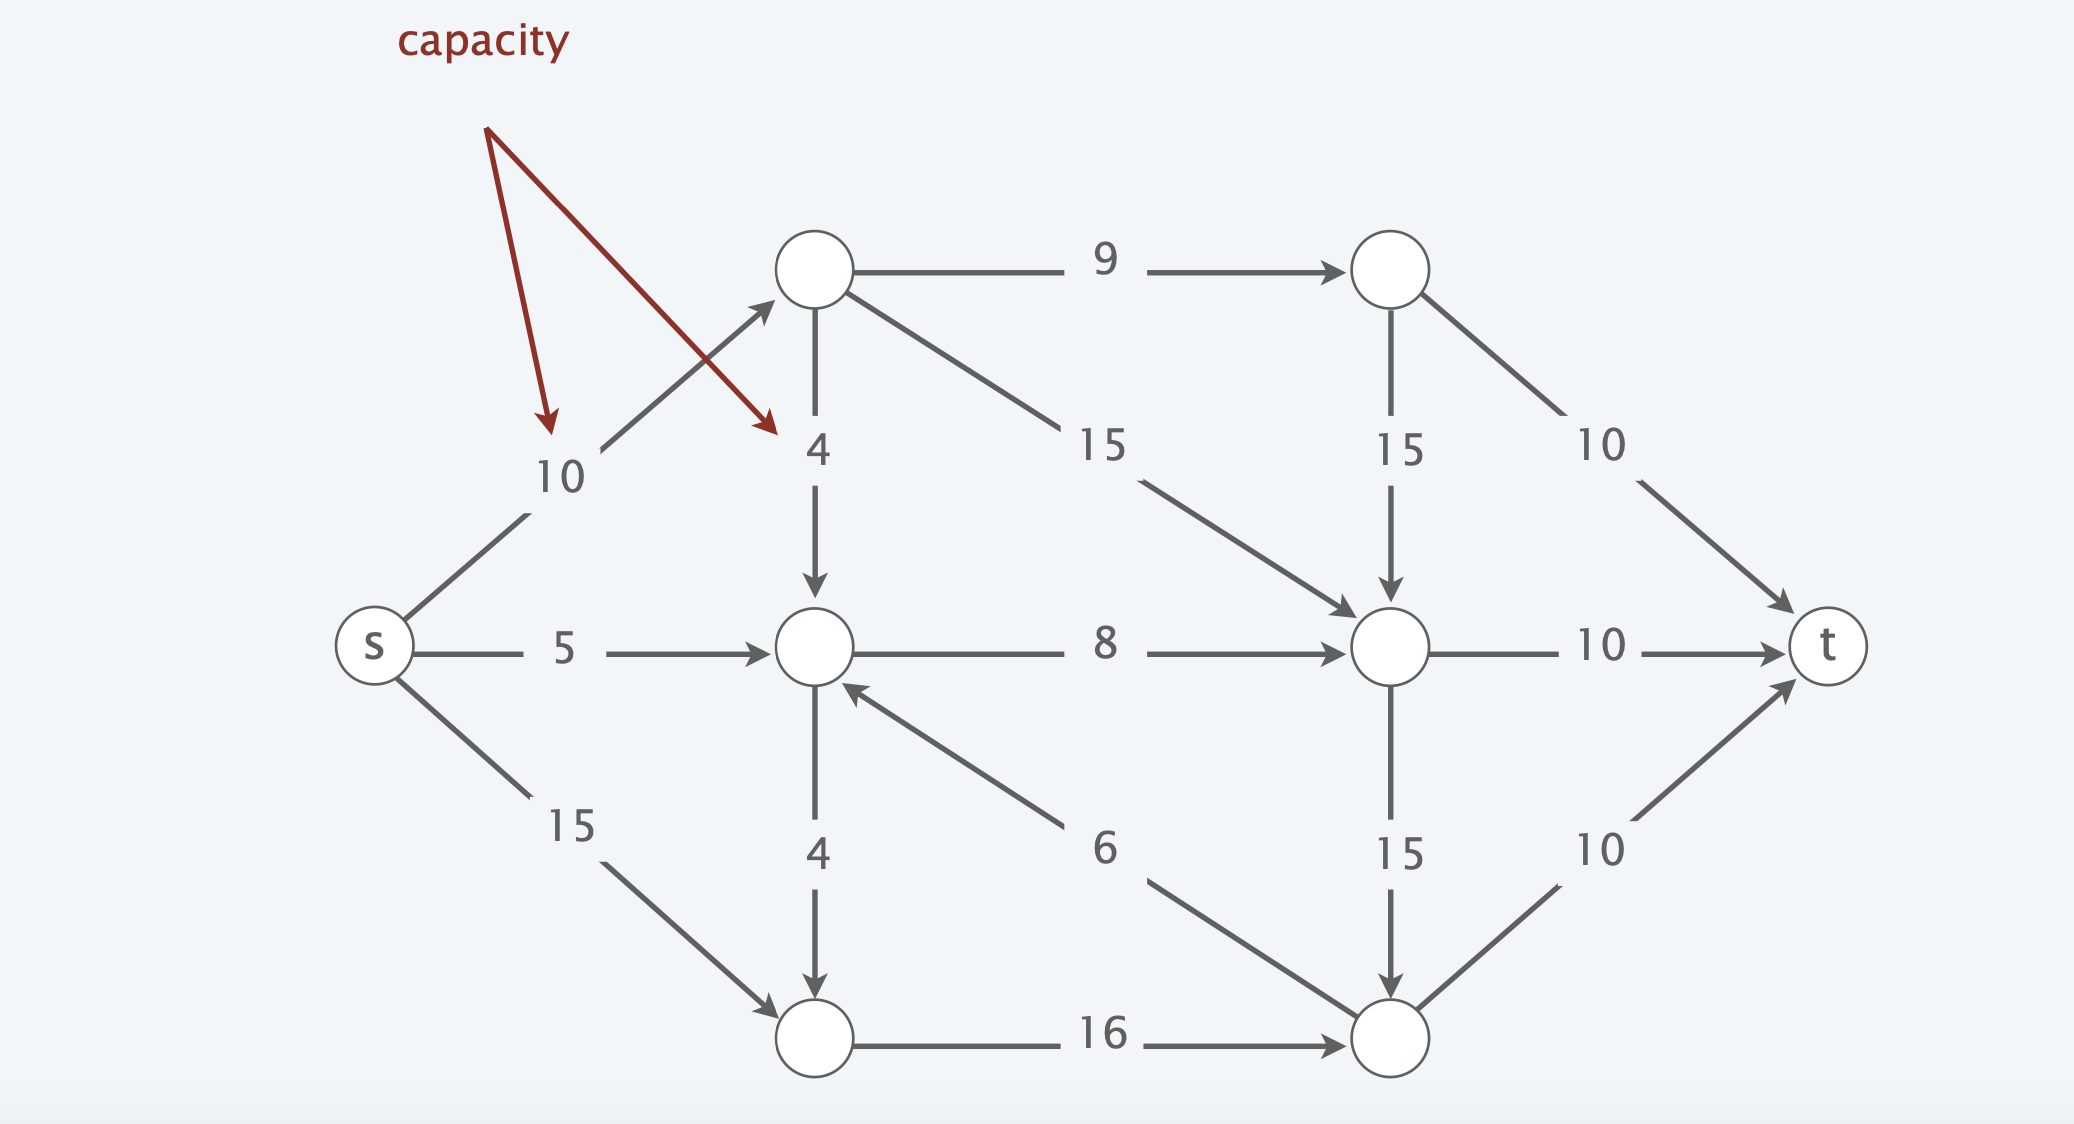
\includegraphics[width=0.5\textwidth ]{network1}
		\caption{An instance of network flow.}
\end{figure}

\subsection{The Maximum Flow Problem}
An $s \rightarrow t$ is a function f that satisfies:

\[ \forall e \in E: \; 0 \leq f(e) \leq c(e) \; (capacity)\] 

\[ \forall v \in V - \{s, t\}: \sum_{e \; out \; of \; v}^{} f(e) = \sum_{e \; into \; v}^{} f(e) \; (flow \; conservation)\]

The maximum flow problem, aim at maximizing the flow function, while respecting the constraint above.

\subsection{The maximum flow/ minimum cut relationship}

\begin{itemize}

\item{Residual Graph}

\begin{figure}[H]
		\centering
		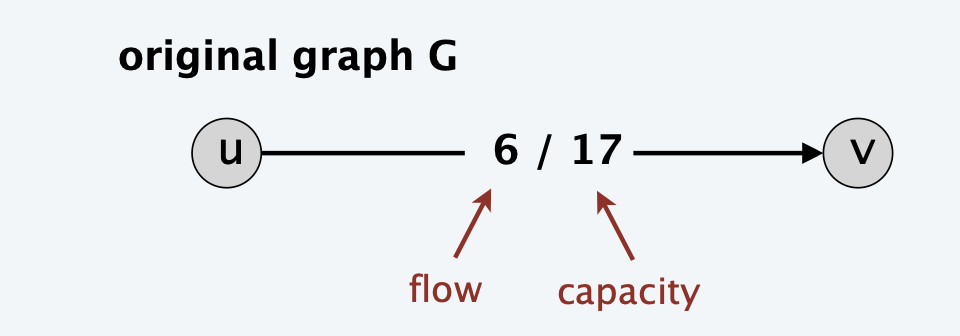
\includegraphics[width=0.3\textwidth ]{residual2}
		\caption{The orignal flow}
\end{figure}

\begin{figure}[H]
		\centering
		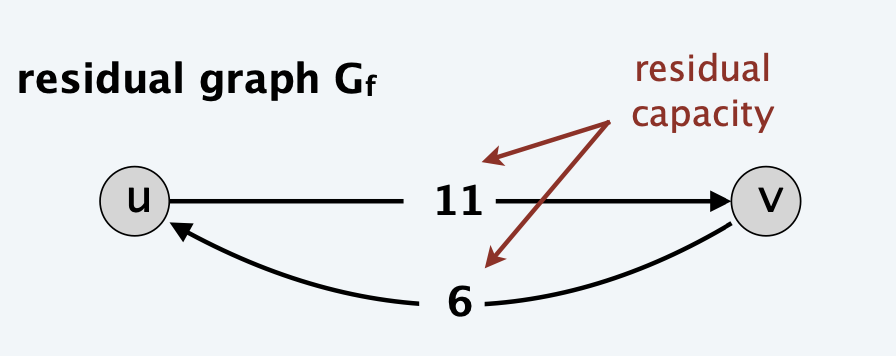
\includegraphics[width=0.3\textwidth ]{residual1}
		\caption{The residual edge.}
\end{figure}

The residual graph G is simply the graph resulting upon applying the residual transformation $\forall e \in E$

\item{Augmenting Path}\\
An augmenting path is a simple $s \leftarrow t$ path P in the residual graph $G_{f}$, The bottleneck capacity of an augmenting P is the minimum residual capacity of any edge in P.

\item {Flow value Lemma}\\
Let f be any flow and let (A, B) be any cut. Then, the net flow across (A, B) equals the value of f:

\[ \sum_{e \; out \; of \; A}^{} f(e) = \sum_{e \; into \; A}^{} f(e) = v(f)\]

proof:

\[v(f) = \sum_{e \; outof  \; s}^{} f(e) =  \sum_{v \in A}^{} ( \sum_{e \; out of  \; v}^{} f(e) - \sum_{e \; into  \; v}^{} f(e)) =  ( \sum_{e \; out of  \; A}^{} f(e) - \sum_{e \; into  \; A}^{} f(e))\]

\item {Weak Duality}\\
Let f be any flow and (A, B) be any cut. Then, v( f ) $\leq$ cap(A, B).

proof:

\[v(f) =  \sum_{e \; out of  \; A}^{} f(e) - \sum_{e \; into  \; A}^{} f(e) \leq  \sum_{e \; out of  \; A}^{} f(e) \leq \sum_{e \; out of  \; A}^{} c(e) = cap(A,B)\]

\item {Integrality Theorem}\\
If c(e) $\forall e \in E$ are integers, then there exists a max flow f for which every flow value f(e) is an integer.

\end{itemize}

\begin{claim}
The value of the maximum flow equals to the minimum cut, furthermore, when the flow is maximized there are no augmenting path left.
\end{claim}\\

\begin{proof}
If there exists a cut (A, B) such that cap(A, B) = val(f),there is no augmenting path with respect to f, so f is a max-flow. 
\end{proof}

\subsection{Ford-Fulkerson Algorithm}
It's a simple greedy approach algorithm: basically we start with a f(e) = 0 $\forall e \in E$, then we will find all the augmenting path in G(V,E) until there are no more left, the result is both a maximum flow and an min-cut.\\

\begin{algorithm}[H]
\SetAlgoLined
\small
\KwIn{$G$ directed graph \; $s$ source node of the flow, $t$ sink of the flow.}
\KwOut{$S$ containing all the paths that maxes the maximum flow. $\leftarrow$ t}

\BlankLine
	

\BlankLine

\caption{FordFulkerson(G,s,t):}
\end{algorithm}

\begin{claim}
The Ford-Fulkerson complexity is $\mathcal{O}(|E|f^{*})$ 
\end{claim}\\

\begin{proof}
the algorithm terminates only when there are no more augmenting paths on G and by definition there is no more flow in the residual net $f^{*}$. Since the algorithm needs to check all the augmenting paths until there are no more left, the execution is closely releated on how many augmenting paths are in G.
\end{proof}

\subsection{Matching and Bipartite Matching}

\emph{Formal definition}: Given an undirected graph G = (V, E) a subset of edges $M \subseteq E$ is a matching if each node appears in at most one edge in M, the maximum matching is a max cardinality matching.

\begin{figure}[H]
		\centering
		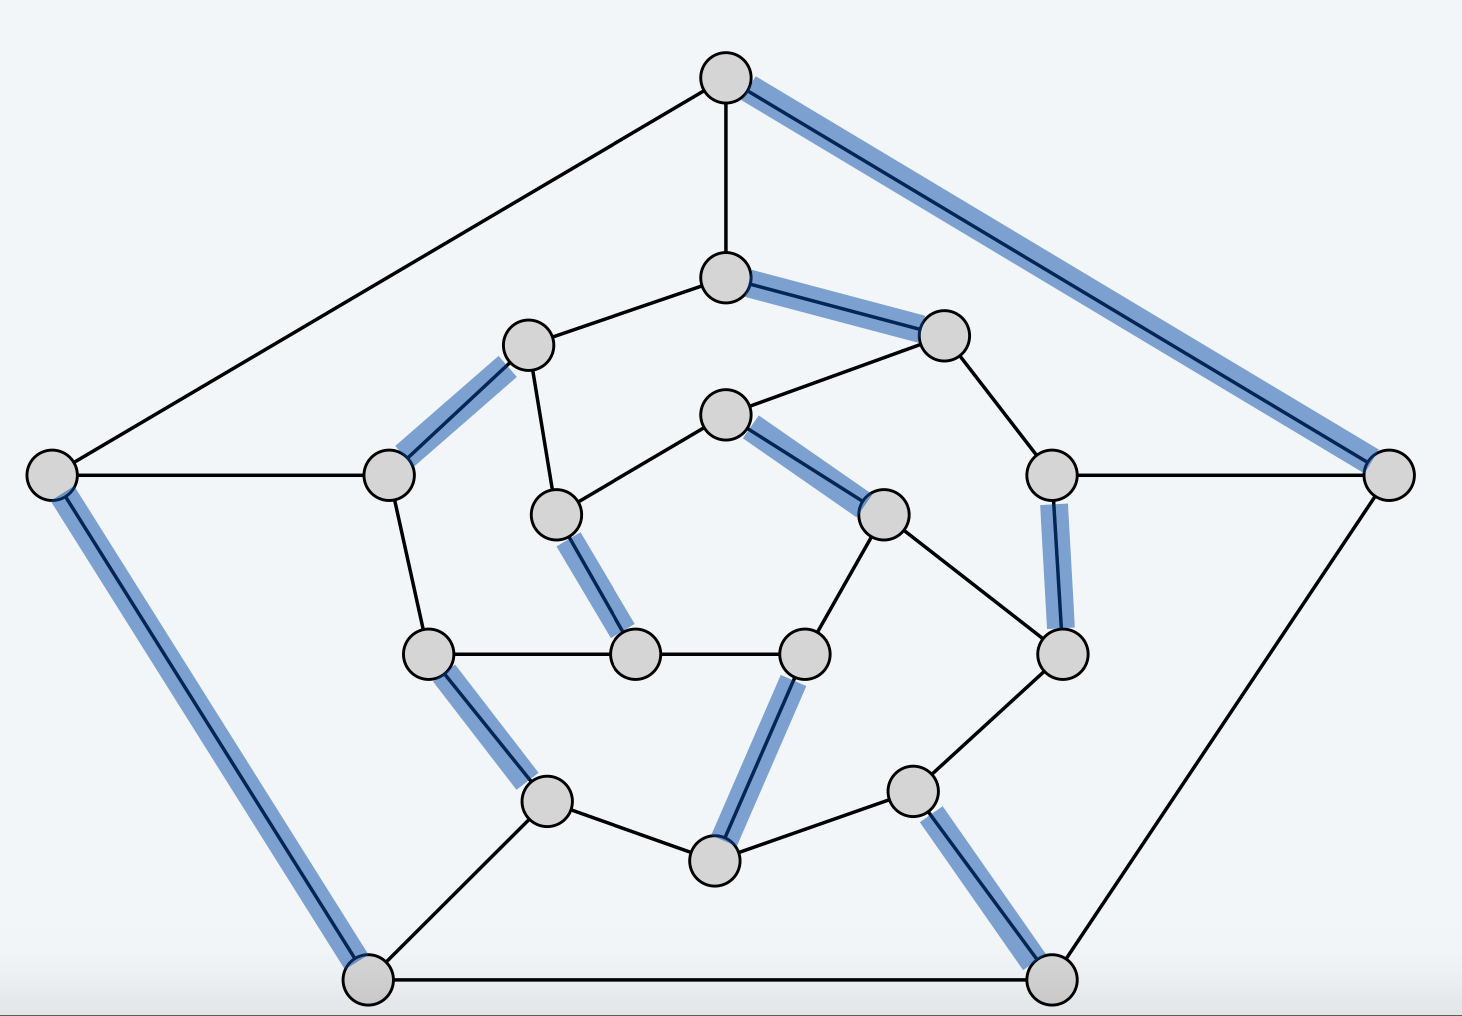
\includegraphics[width=0.5\textwidth ]{matching}
		\caption{The maximum matching in a Graph G}
\end{figure}

\emph{Formal definition}: A graph G is bipartite if the nodes can be partitioned into two subsets L (Left) and R (Right) such that every edge connects a node in L to one in R, a bipartite matching G = (L $\cup$ R, E), find a max cardinality matching.

\begin{figure}[H]
		\centering
		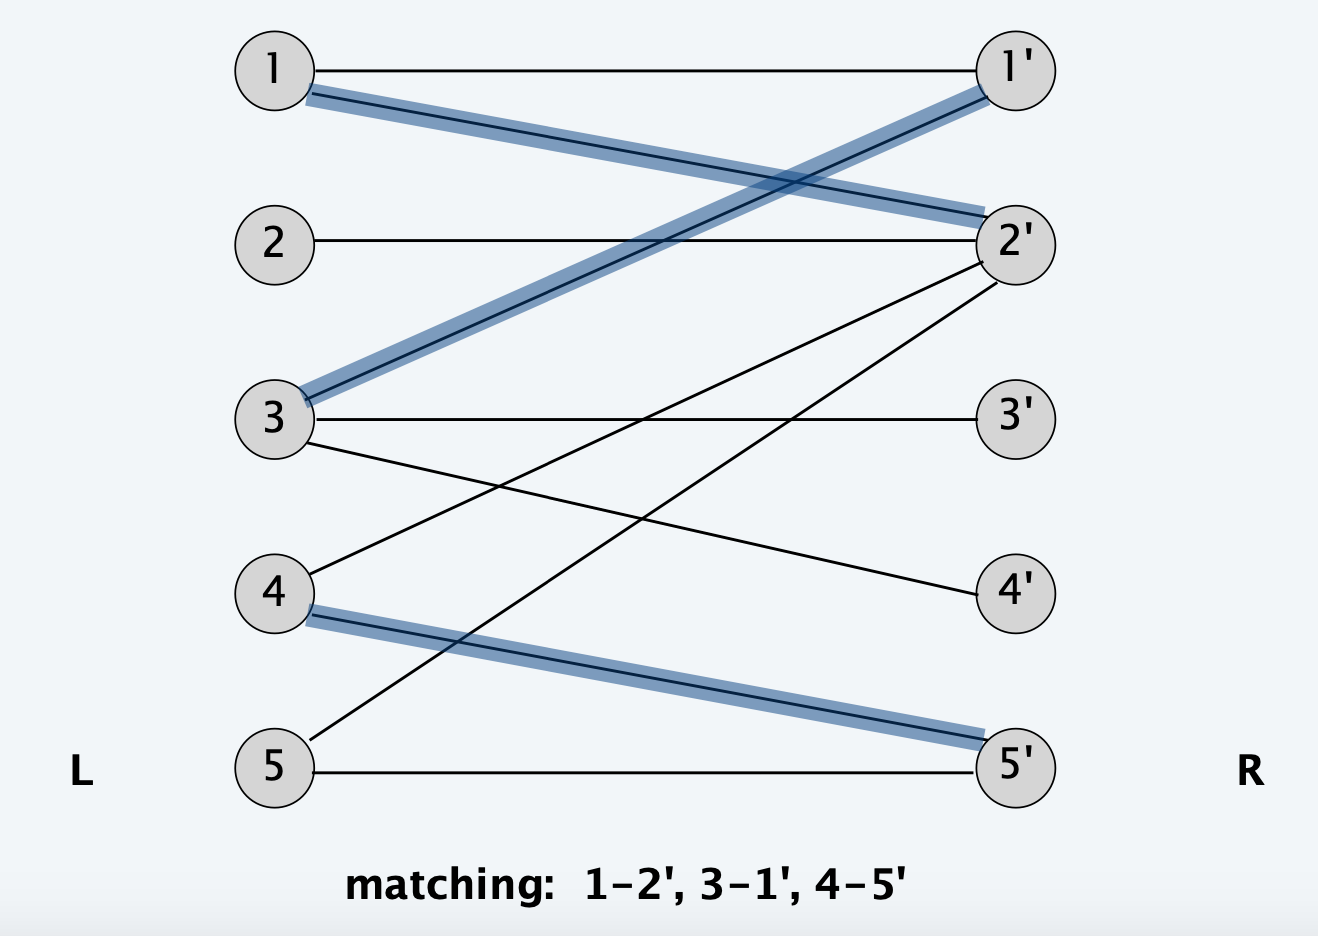
\includegraphics[width=0.5\textwidth ]{bmatching}
		\caption{The maximum bipartite matching in a Graph G}
\end{figure}


\emph{Hall Theorem}: Let S be a subset of nodes, and let N(S) be the set of nodes adjacent to nodes in S, Let $G = (L \cup R, E)$ be a bipartite graph with $|L| = |R|$. G has a perfect matching iff $|N(S)| \geq |S|$ for all subsets $S \subseteq L$.\\

\clearpage

\emph{Proof}: Suppose G does not have a perfect matching: formulate a max flow problem and let (A, B) be min cut in G', by max-flow min-cut theorem: $cap(A, B) < | L |$.\\
Define LA=$L\cap A, LB=L \cap B, RA=R \cap A$, so the cap(A, B) = $| LB | + | RA |$. Since min cut can't use $\infty$ edges: $N(LA) \subseteq RA \; with \; |N(LA)| \leq |RA|$ = $cap(A,B) – |LB| < |L| – |LB| = |LA|$ so S=LA.

\begin{figure}[H]
		\centering
		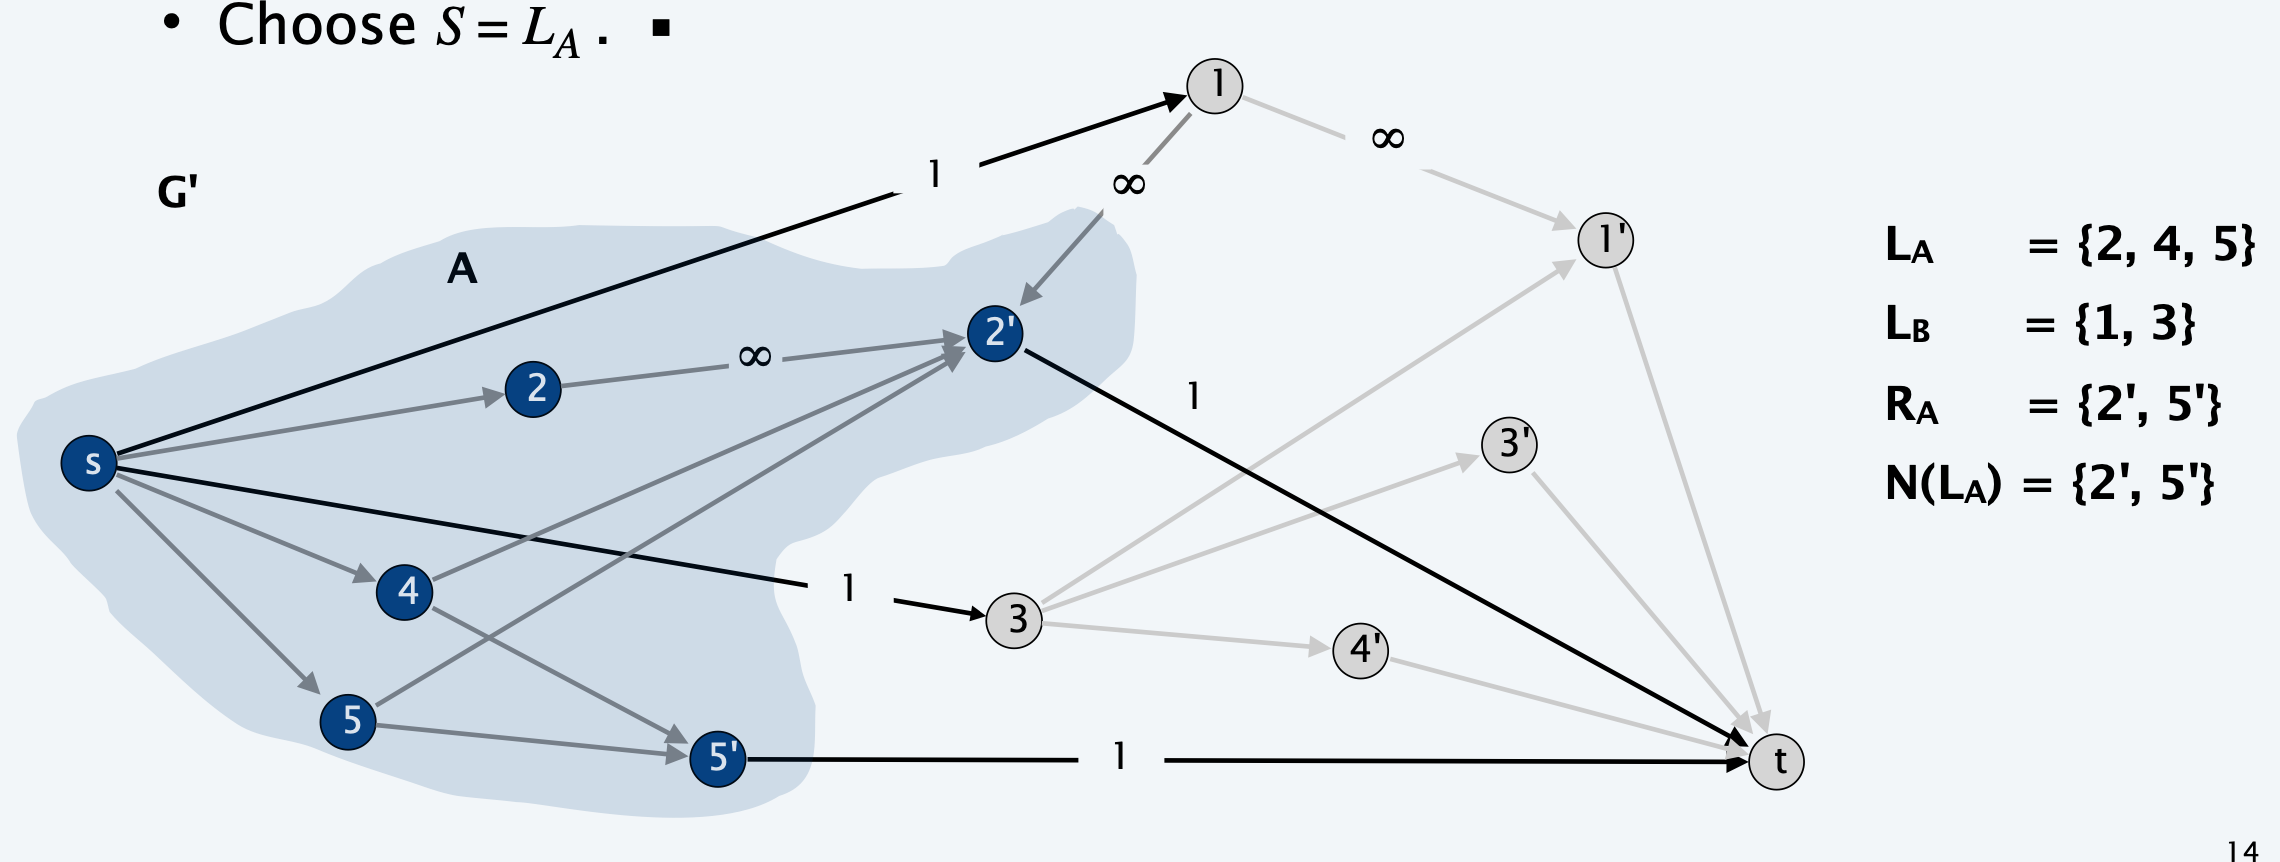
\includegraphics[width=0.8\textwidth ]{hall}
		\caption{}
\end{figure}


\begin{claim}
The max cardinality of a matching in G = value of max flow in G'.
\end{claim}\\

\begin{proof}
First we need to build $G_{'} = (L \cup R \cup \{s, t\}, E^{'} )$ , direct all edges from L to R and give them unit capacity, then connect s to all $e \in L$ and t to all $e \in R$ with edges with infinite capacity, using the integrality theorem we know that the flow can assume only value 0-1. Finally consider the set of edges from L to R with f (e) = 1, each node in L and R participates in at most one edge in M, with with f (e) = 1 so $| M | = k$: considering the  cut ($L \cup s, R \cup t$).
\end{proof}

\subsection{Edge Disjointed Paths}
\emph{Definition}:Two paths are edge-disjoint if they have no edge in common.\\\\
\emph{Edge Disjointed Problem}: Given a digraph G = (V, E) and two nodes s and t, find the max number of edge-disjoint $s \Rightarrow t$ paths.


\begin{figure}[H]
		\centering
		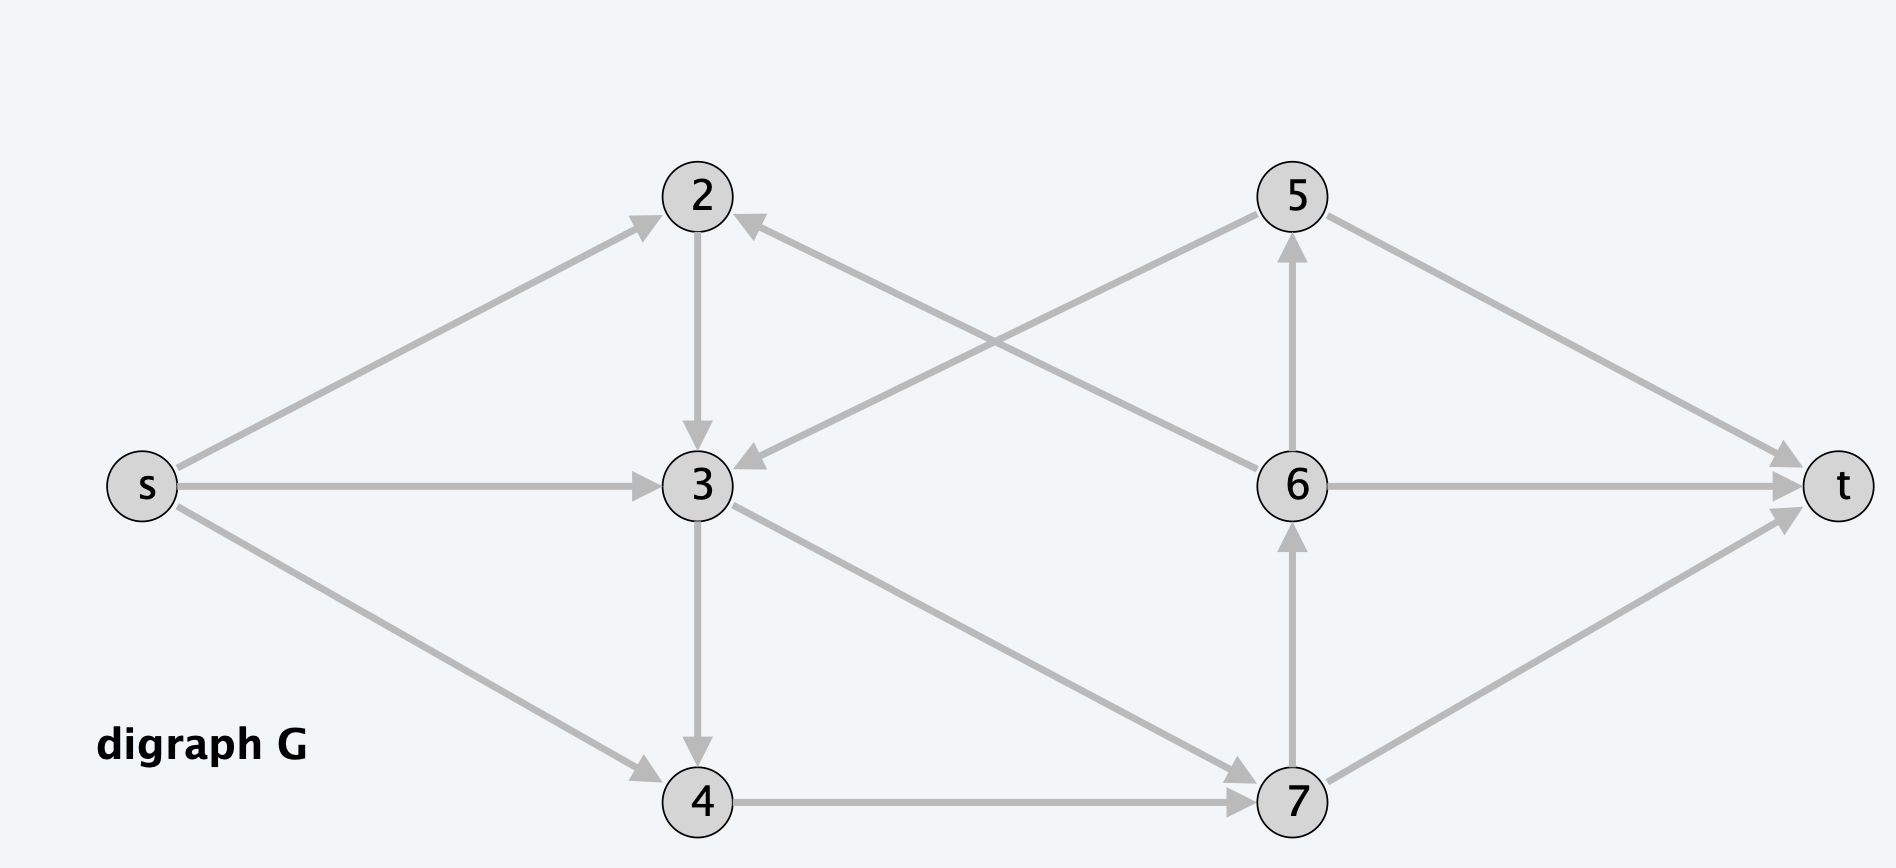
\includegraphics[width=0.6\textwidth ]{disjointed}
		\caption{Instance of the Disjointed Path problem}
\end{figure}

\begin{claim}
Given a digraph G=(V,E) with $c(e) = 1,\; \forall e \in E$ the max number edge-disjoint $s \Rightarrow t $ paths equals value of max flow.
\end{claim}\\

\begin{proof}
Suppose max flow value is k: Integrality theorem $ \Rightarrow $  there exists 0-1 flow f of value k. Now Consider edge (s, u) with f(s, u) = 1.\\
By conservation, there exists an edge (u, v) with f(u, v) = 1 continue until reach t, always choosing a new edge, the solution produces k (not necessarily simple) edge-disjoint paths.
\end{proof}\\

\begin{figure}[H]
		\centering
		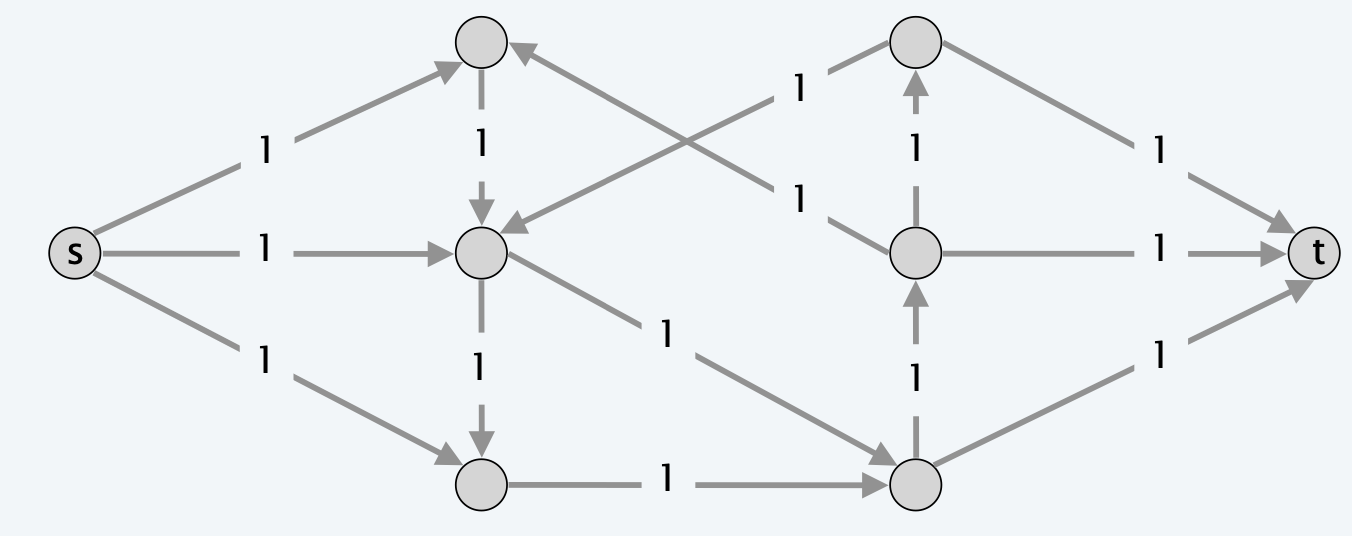
\includegraphics[width=0.6\textwidth ]{maxFlowDisjointed}
		\caption{Instance of the Disjointed Path problem}
\end{figure}

\begin{claim}
\emph{Manger's Theorem}: The max number of edge-disjoint $s \Rightarrow t$ paths is equal to the min number of edges whose removal disconnects t from s.
\end{claim}\\

\begin{proof}
Suppose max number of edge-disjoint paths is k: then value of max flow = k, using the max-flow min-cut theorem $  \Rightarrow $ there exists a cut (A, B) of capacity k. Let F be set of edges going from A to B.
$|F| = k$ and disconnects t from s.
\end{proof}\\

The Manger's theorem can even be applied to undirected graphs: (it's always possible to transform an undirected graph to directed by simply replacing every edge (u,v) with 2 direct edges (u,v) and (v,u)), then the formulation and proof is the same as above.

\subsection{Circulation With demands}
Given a digraph G = (V, E) with nonnegative edge capacities c(e) and node supply and demands d(v), a circulation is a function that satisfies:

\[ \forall e \in E: \; 0 \leq f(e) \leq c(e) \; (capacity)\] 

\[ \forall v \in V: \sum_{e \; out \; of \; v}^{} f(e) = \sum_{e \; into \; v}^{} f(e) = d(v) \; (flow \; conservation)\]

\begin{figure}[H]
		\centering
		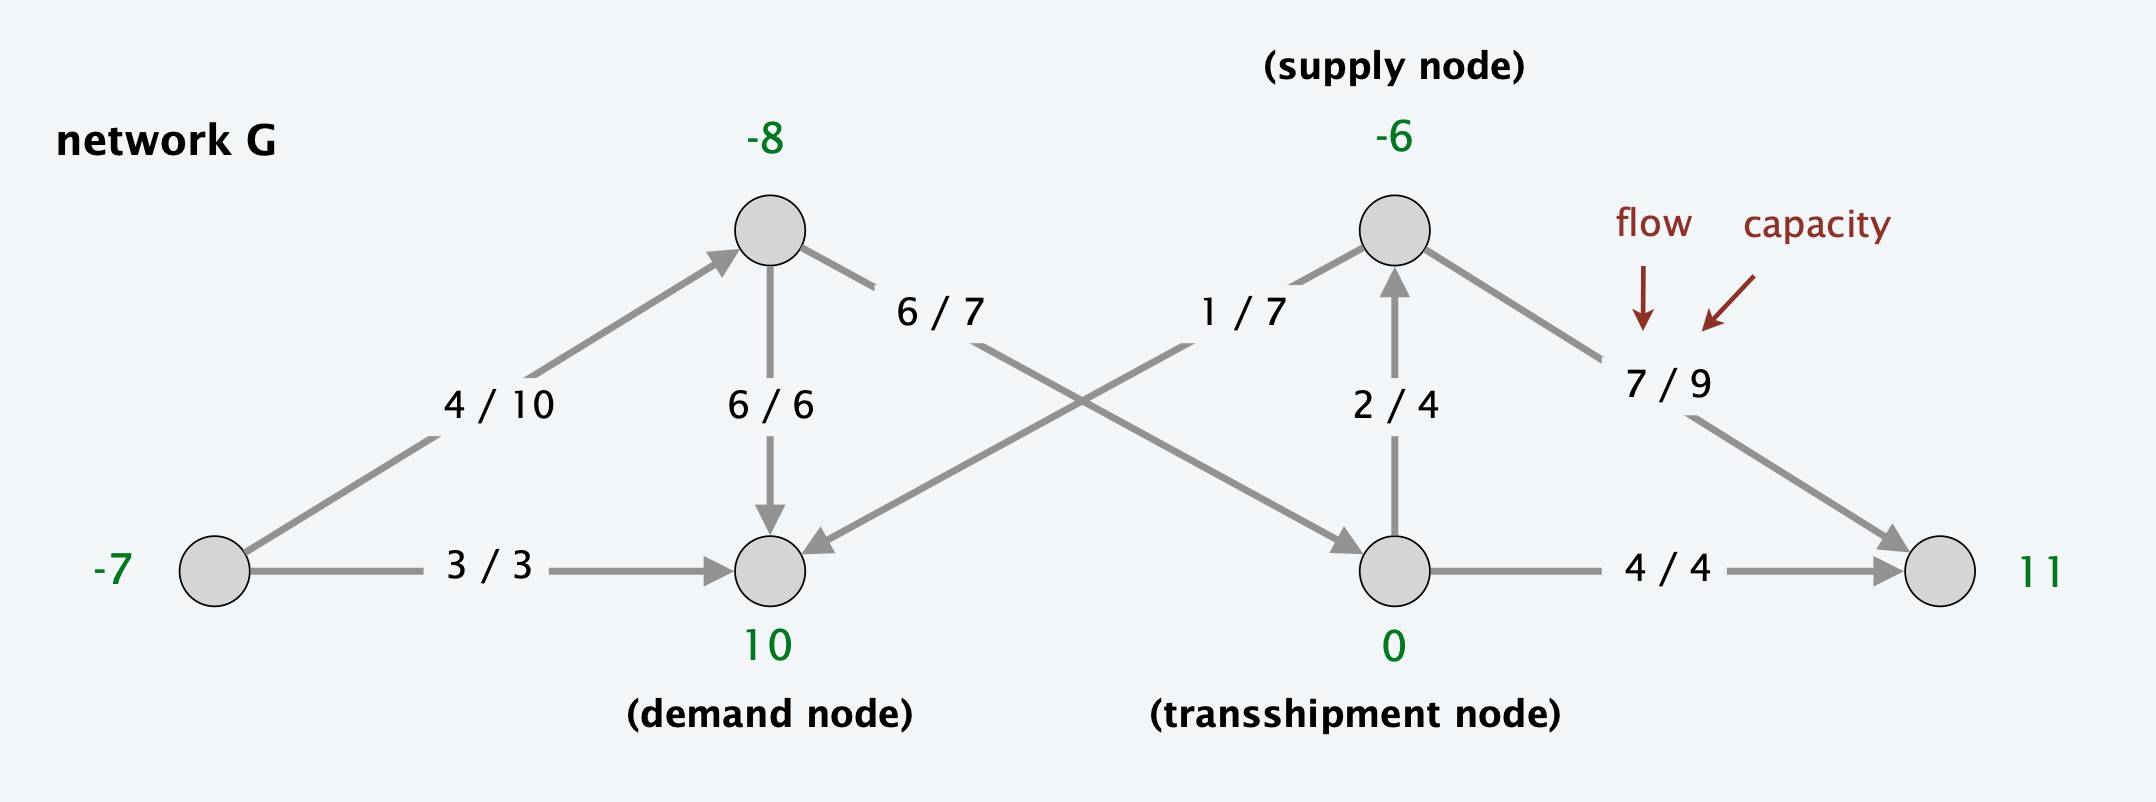
\includegraphics[width=0.6\textwidth ]{circulation}
		\caption{Instance of the Circulation problem}
\end{figure}

In order to transform the circulation into a flow problem we need to connect the source s to each node with $d(v) < 0$ and t with each node with $d(v) > 0$.\\
The original Graph G has a circulation if G' has a max flow of value:
\[ \sum _{v \: in \; d(v) > 0 } d(v) = \sum _{v \; in \; d(v) < 0} - d(v)\]

\begin{figure}[H]
		\centering
		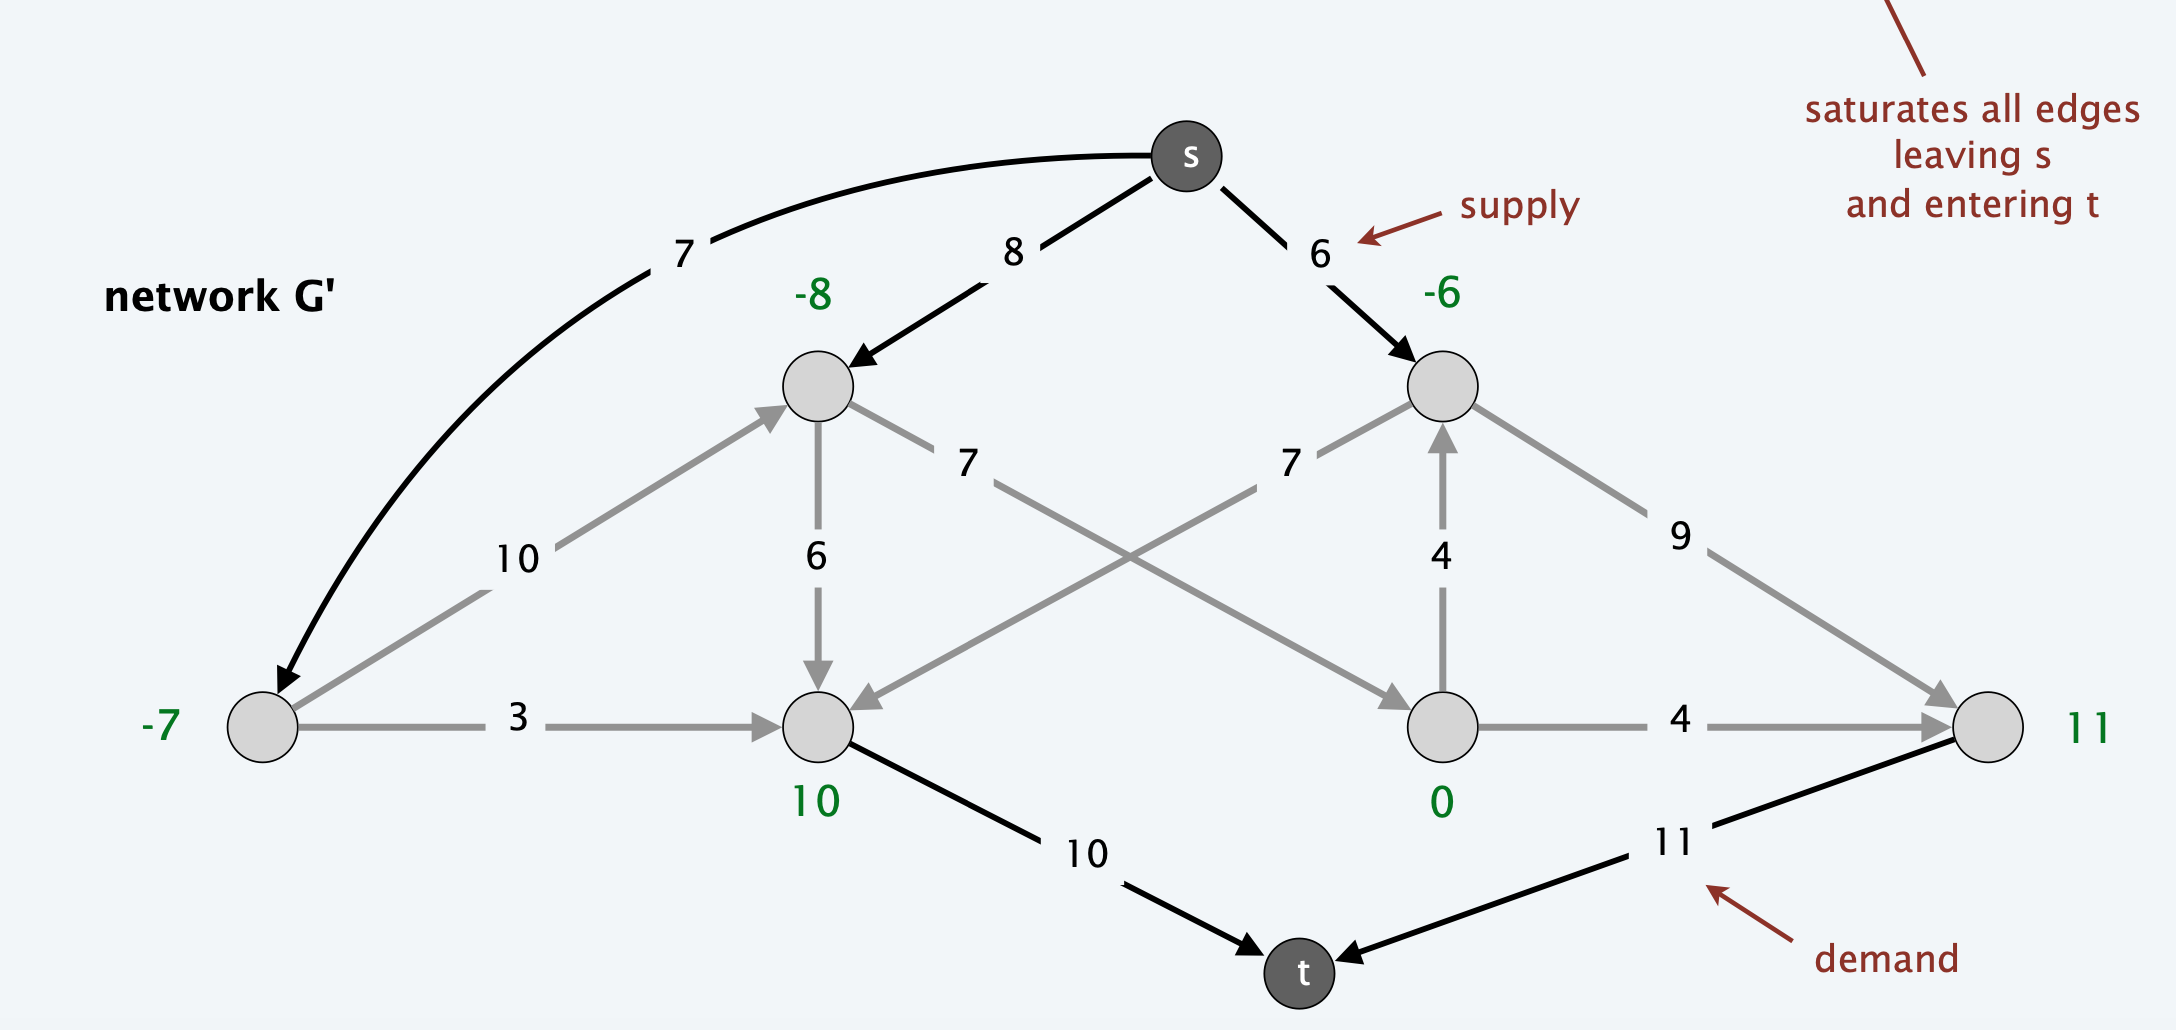
\includegraphics[width=0.6\textwidth ]{maxFlowCirculation}
		\caption{Instance of the Circulation problem with source and sink}
\end{figure}

\begin{claim}
Given (V, E, c, d), there does not exist a circulation iff there exists a node partition (A, B) such that $\sum _{v \in B} d(v) > cap(A, B).$
\end{claim}\\

\begin{proof}
By construction, simply looking at the minimum cut of G'.
\end{proof}\\

\emph{Circulation with Lowerbound:}\\\\
Same as before, the problem is the following: Given (V, E, l, c, d), (with l(e) that express lowerbound on $\forall e \in E$) does exist a feasible circulation?\\
The solution is the same as before, modeling the lowerbound problem as a circulation with demands:

\begin{figure}[H]
		\centering
		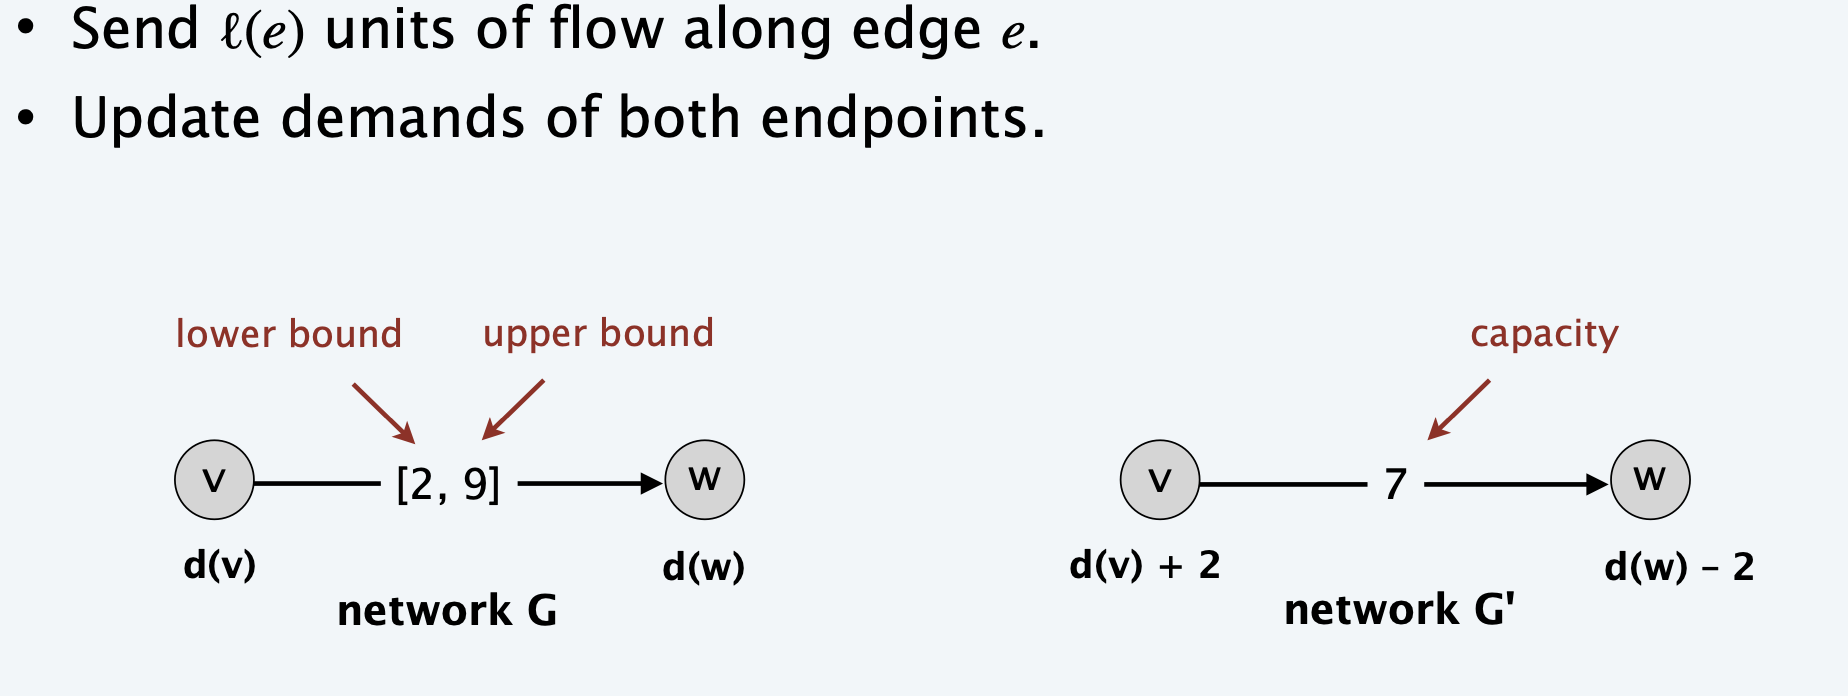
\includegraphics[width=0.6\textwidth ]{lowerbound}
		\caption{Instance of the Circulation problem with lowerbound}
\end{figure}

\begin{claim}
There exists a circulation in G iff there exists a circulation in G'. Moreover, if all demands, capacities, and lower bounds in G are integers, then there is a circulation in G that is integer-valued.
\end{claim}\\

\begin{proof}
By construction: f(e) is a circulation in G iff f '(e) = f (e) – l(e) is a circulation in G'.
\end{proof}\\

\subsection{Survey Design}

Design survey asking n consumers about n products but you can only survey consumer i about product j if they own it, you can ask consumer i between ci and ci' questions and only between pj and pj' consumers about product j, the goal is to design a survey that meets these specs, if possible.\\

\emph{Solution}: Model as circulation problem with lower bounds:add edge (i, j) if consumer j owns product i, connect every product to t and every client to s and lastly connect t to s: the integrality circulation is a feasible survey design.

\begin{figure}[H]
		\centering
		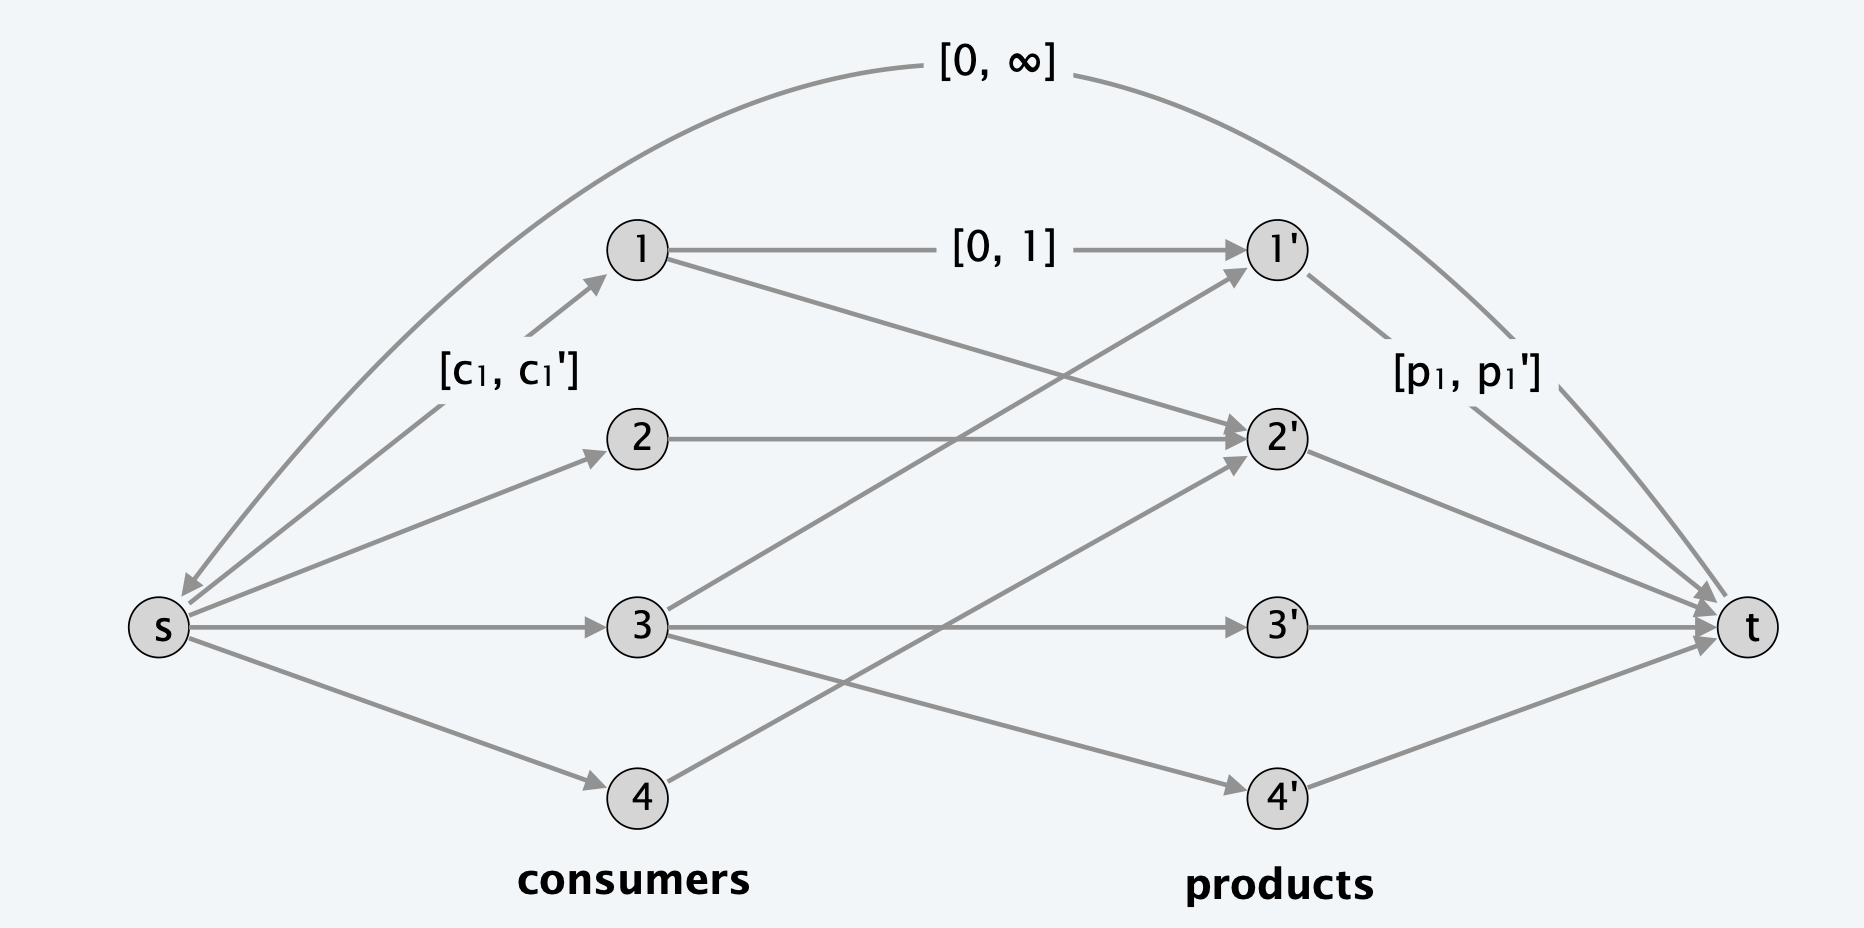
\includegraphics[width=0.6\textwidth ]{survey}
		\caption{Instance of the Survey Problem}
\end{figure}

\subsection{Airline Scheduling}

Airline Scheduling is Complex computational problem faced by nation's airline carriers. Produces schedules that are efficient in terms of: equipment usage, crew allocation, customer satisfaction
and in presence of unpredictable issues like weather, breakdowns.\\
The solution proposed below is a "toy problem" because we can: reusing flight multiple times, each
flight i leaves origin $o_{i}$ at time si and arrives at destination di destination at time $f_{i}$.The goal is to minimize number of flight crews.

\begin{figure}[H]
		\centering
		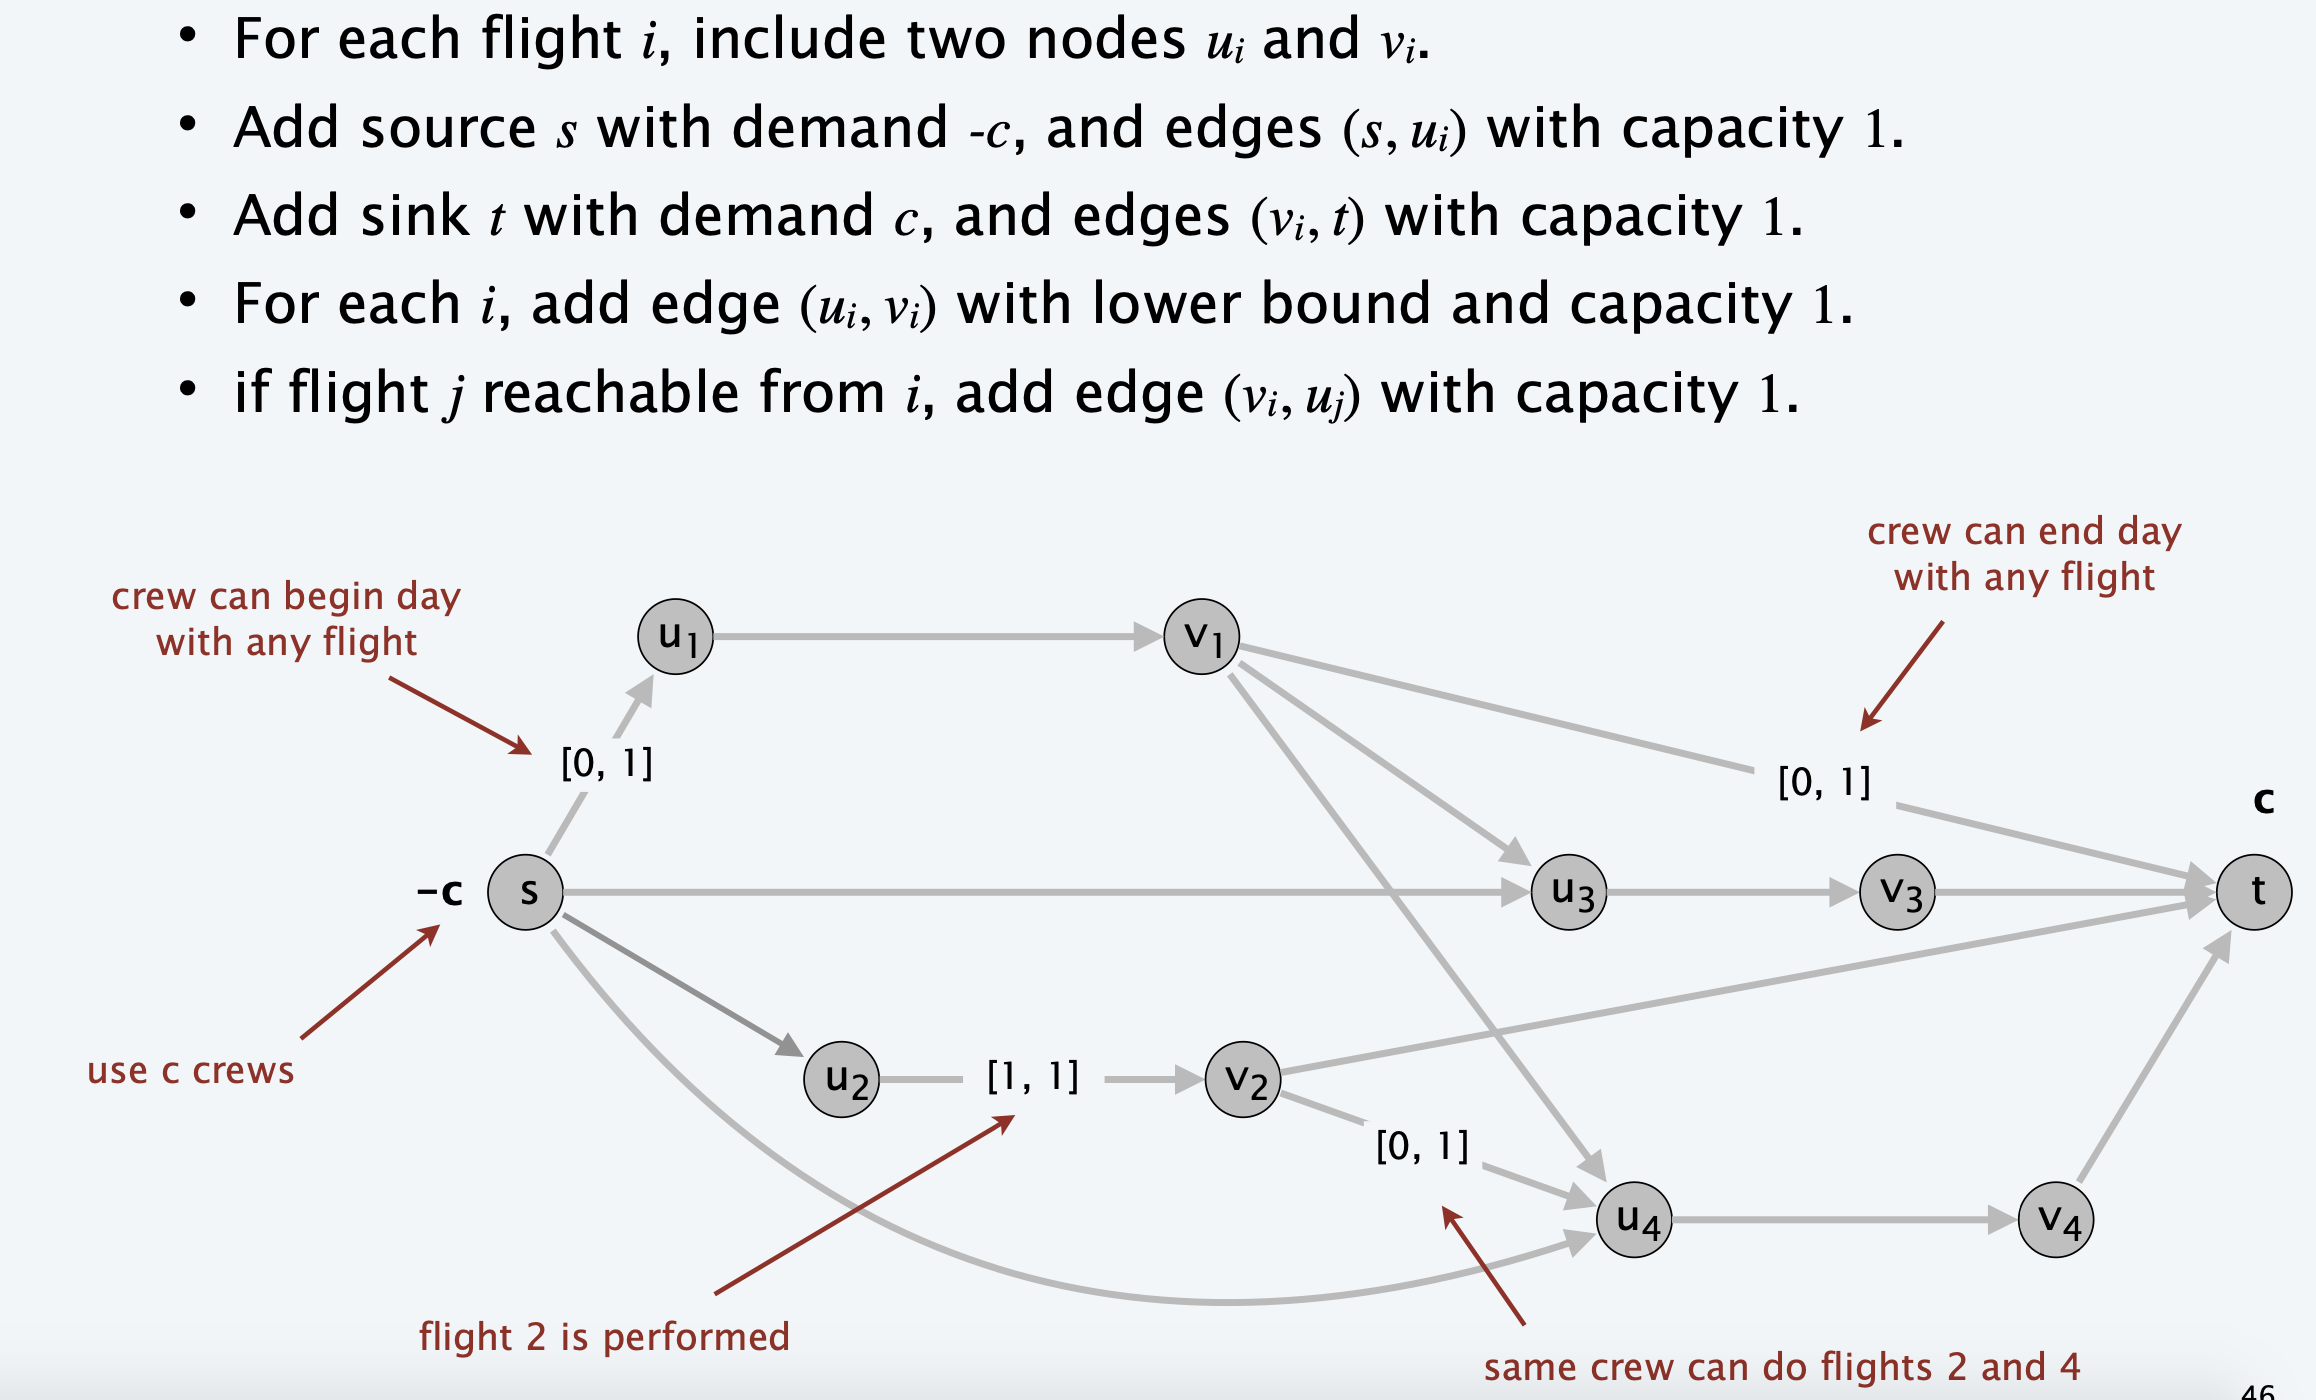
\includegraphics[width=0.6\textwidth ]{airline}
		\caption{Instance of the Airline Problem}
\end{figure}

\begin{claim}
The airline scheduling problem can be solved in $O(k^{3} log k)$ time, with k = number of flights.
\end{claim}

\begin{proof}
The number c (of crews is uknown) we have $O(k)$ nodes and $O(k^{2})$ edges so, at most, k crews are needed and by solving the k-circulation problem with at most, k augmenting paths, we obtain $O(k^{3} log k)$ .
\end{proof}

\subsection{Project Selection}
Having a set of possible projects P : project v has associated revenue $p_{v}$, a set of prerequisites E : if $(v, w) \in E$, cannot do project v unless also do project w. A subset of projects $A \subseteq P$ is feasible if the prerequisite of every project in A also belongs to A. Given a set of projects P and prerequisites E, choose a feasible subset of projects to maximize revenue.

\begin{figure}[H]
		\centering
		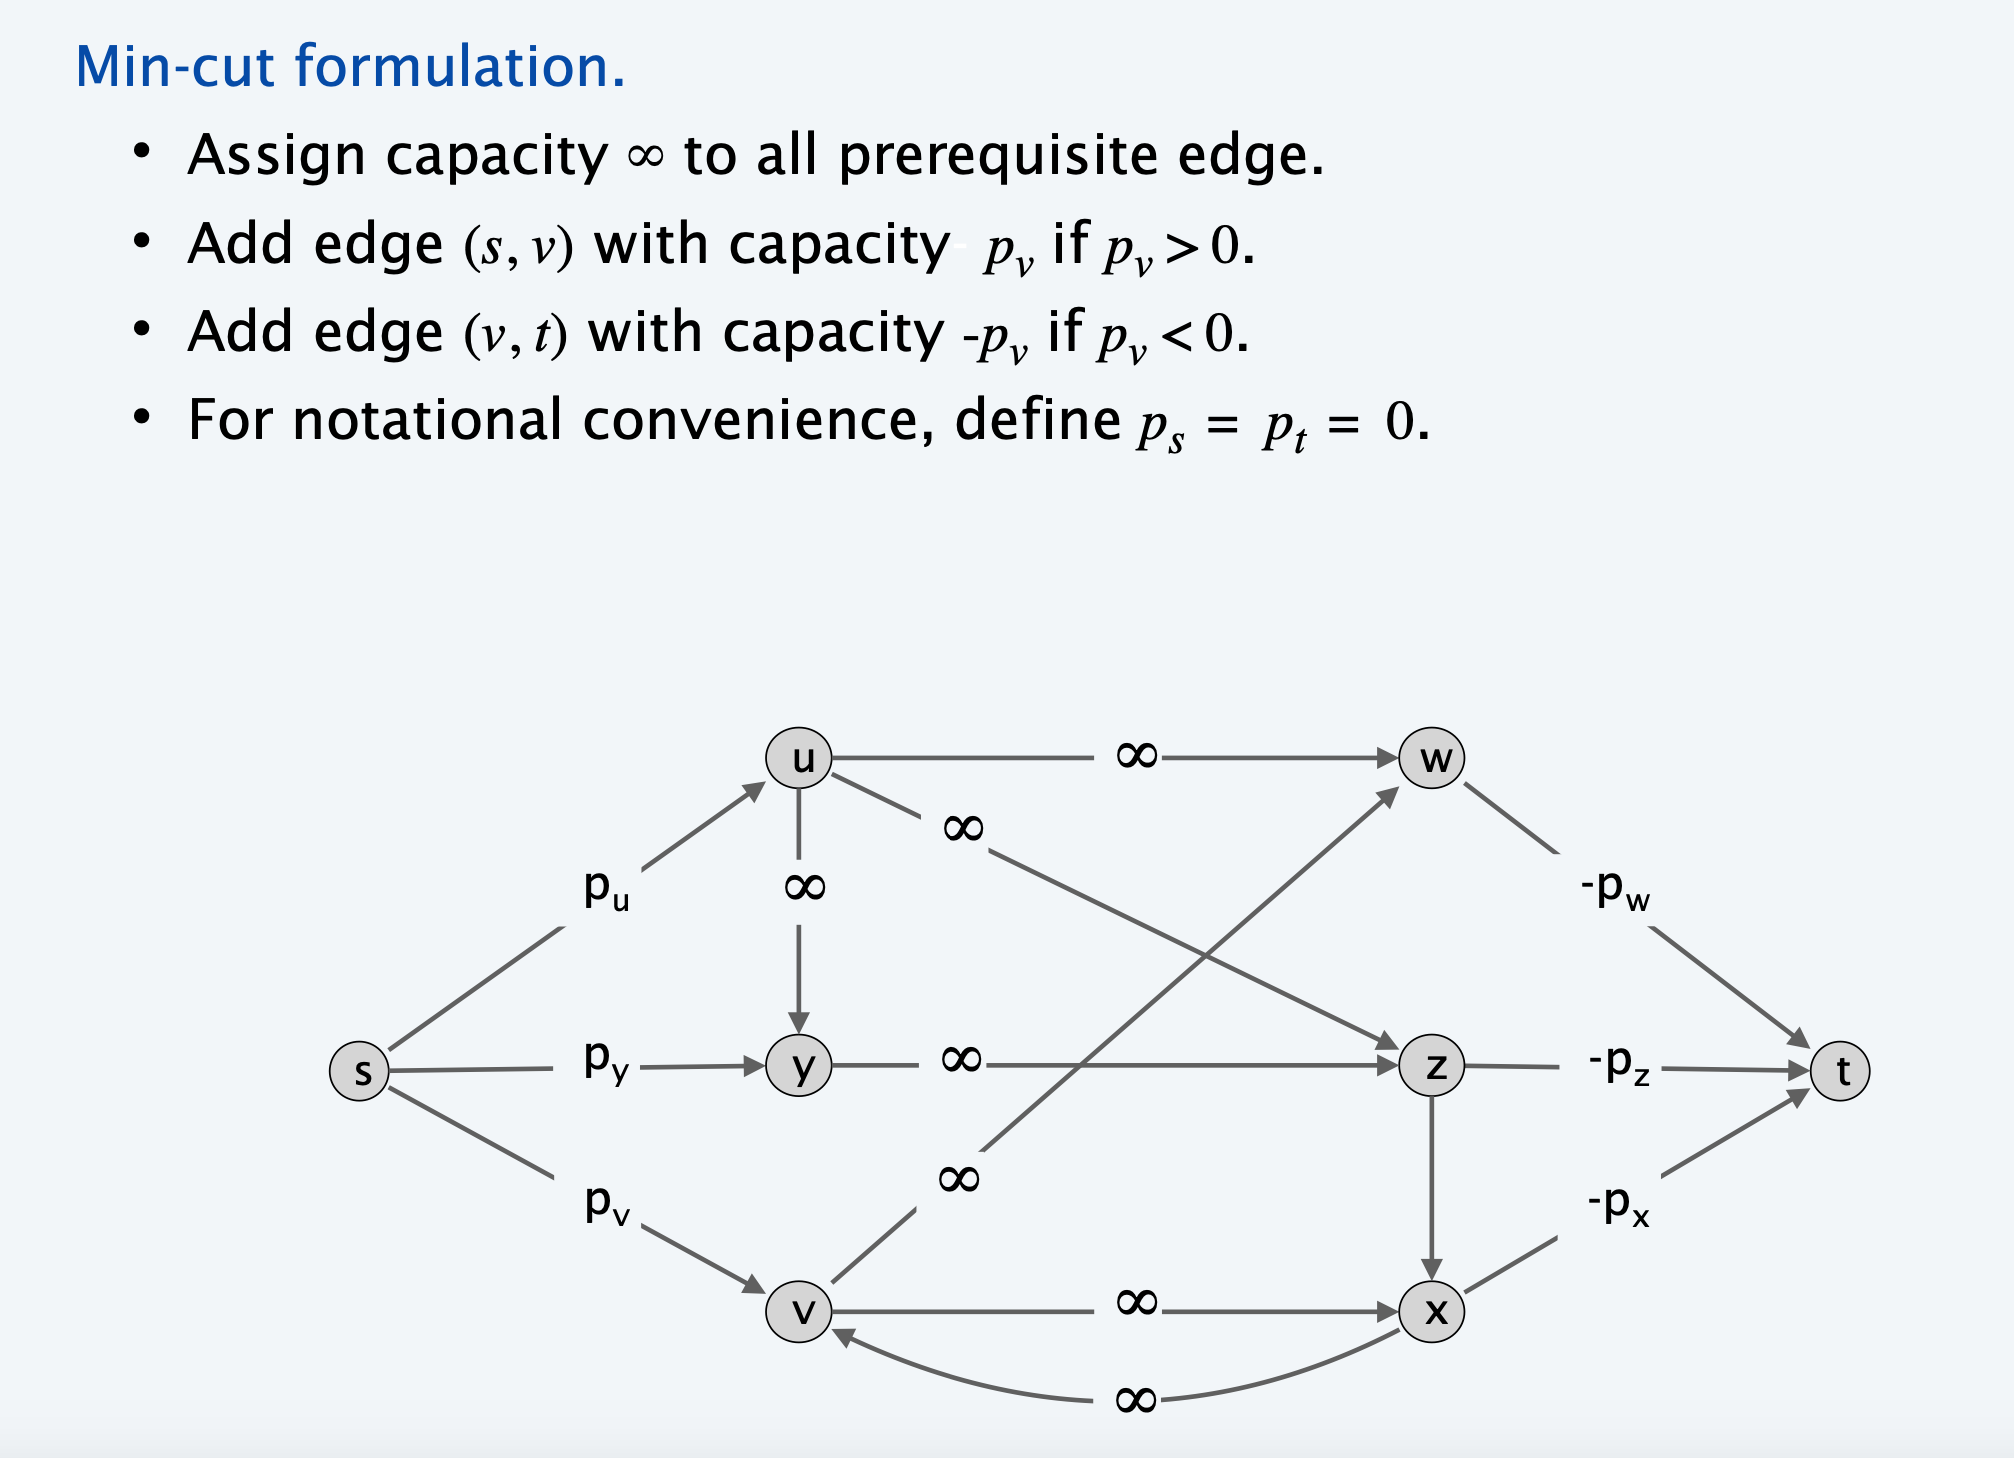
\includegraphics[width=0.6\textwidth ]{projects}
		\caption{Instance of the Projects selection Problem}
\end{figure}

\begin{claim}
(A, B) is min cut iff A − $\{ s \}$ is optimal set of projects.
\end{claim}\\

\begin{proof}
Infinite capacity edges ensure $A − \{ s \}$ is feasible.
\end{proof}

\subsection{Baseball Game}
Which teams have a chance of finishing the season with the most wins? Ex:  Montreal is mathematically eliminated (Montreal finishes with $\leq$ 80 wins but Atlanta has already 83). The answer depends not only on how many games already won and left to play, but on whom they're against.\\So we have a set of teams S, distinguished team $z \in S$, team x has won $w_{x}$ games already and x and y play each other $r_{xy}$ additional times.\\\\
Given the current standings, is there any outcome of the remaining games in which team z finishes with the most (or tied for the most) wins?

\begin{figure}[H]
		\centering
		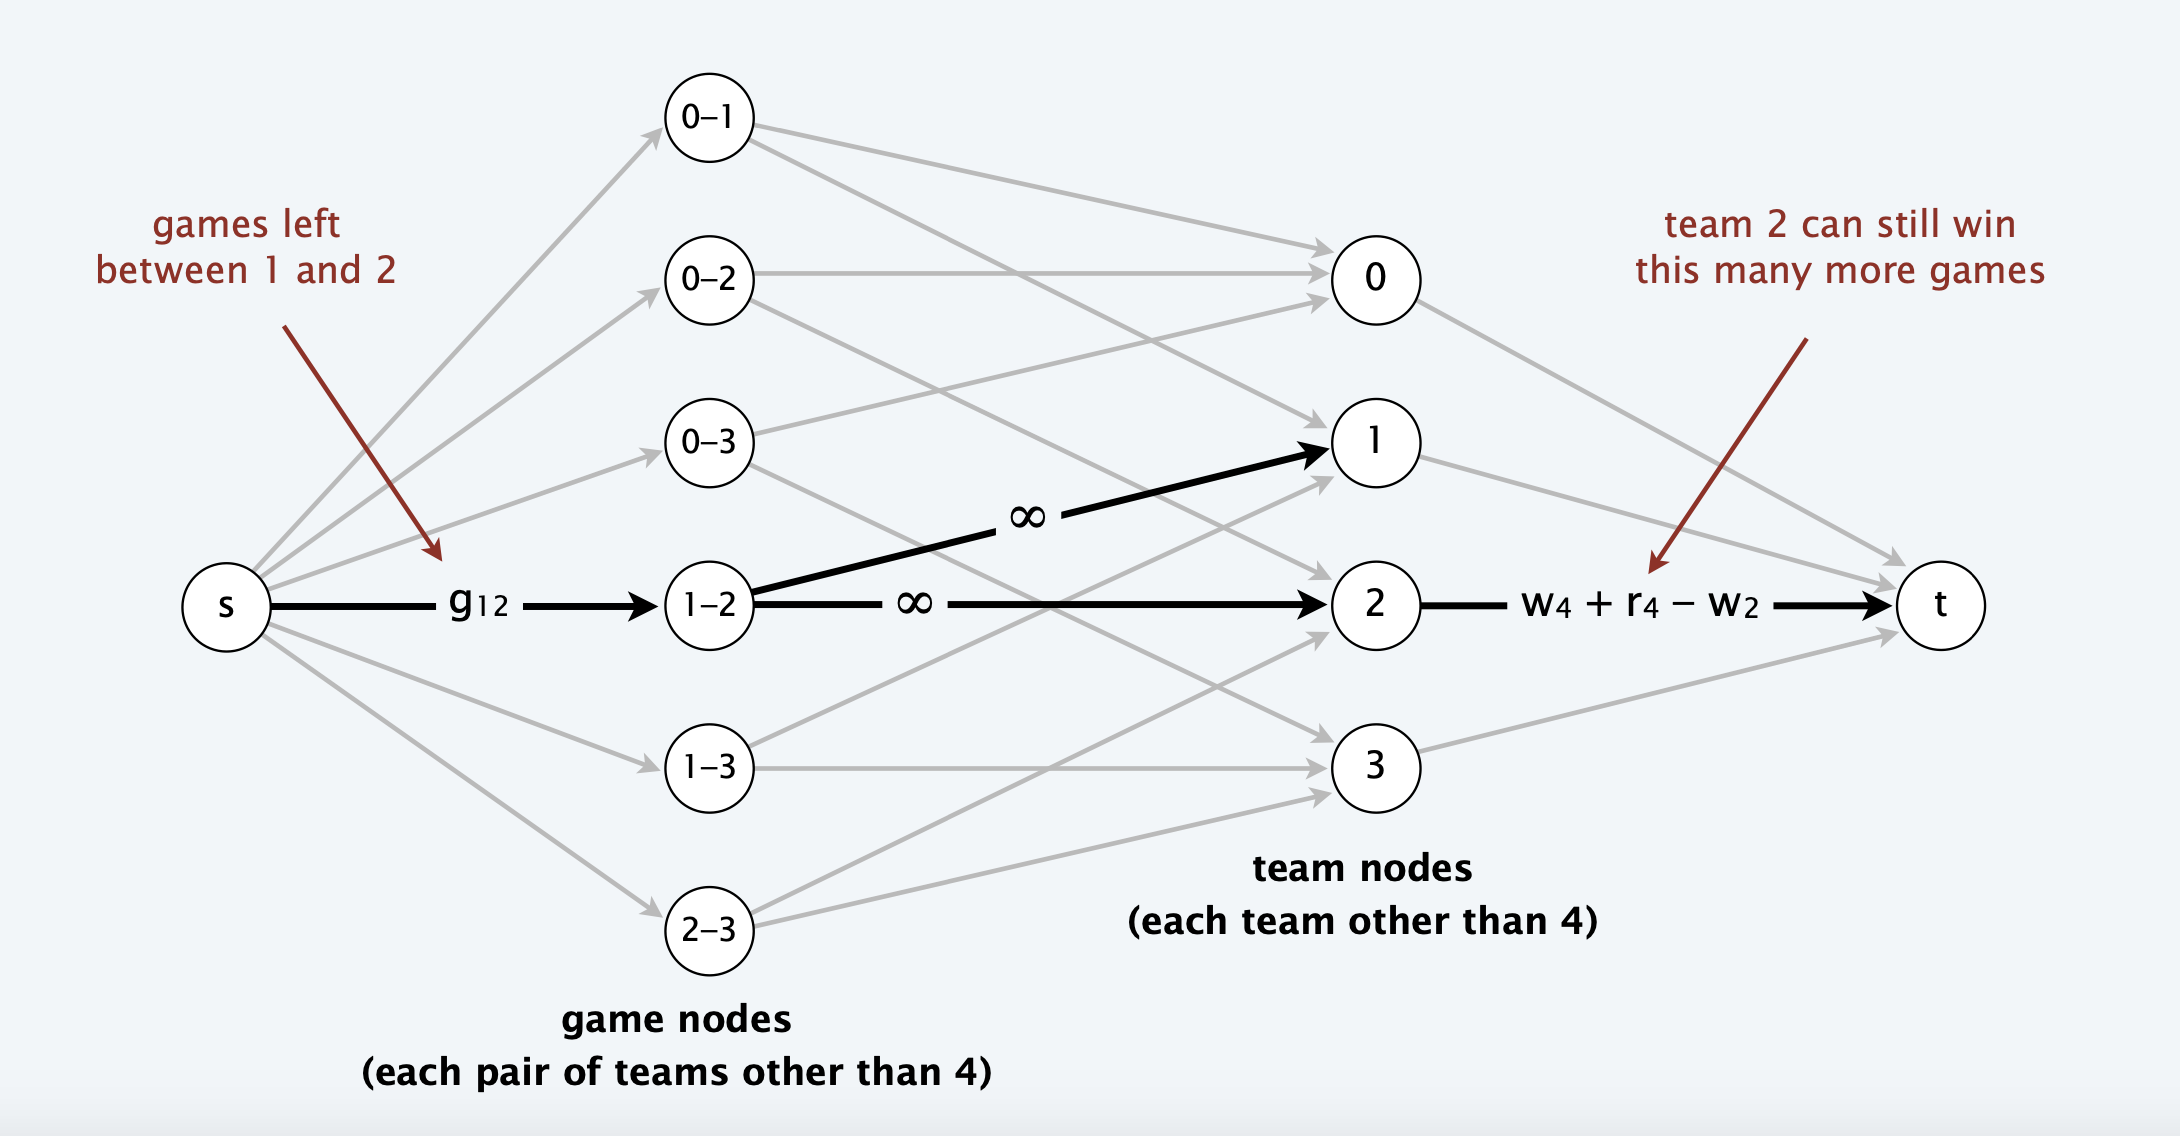
\includegraphics[width=0.6\textwidth ]{baseballFlow}
		\caption{Instance of the Baseball Game Problem}
\end{figure}

\begin{claim}
Team 4 not eliminated iff max flow saturates all edges leaving s.
\end{claim}\\

\begin{proof}
Integrality theorem $\Rightarrow $ each remaining game between x and y added to number of wins for team x or team y, the capacity on (x, t) edges ensure no team wins too many games.
\end{proof}

\begin{figure}[H]
		\centering
		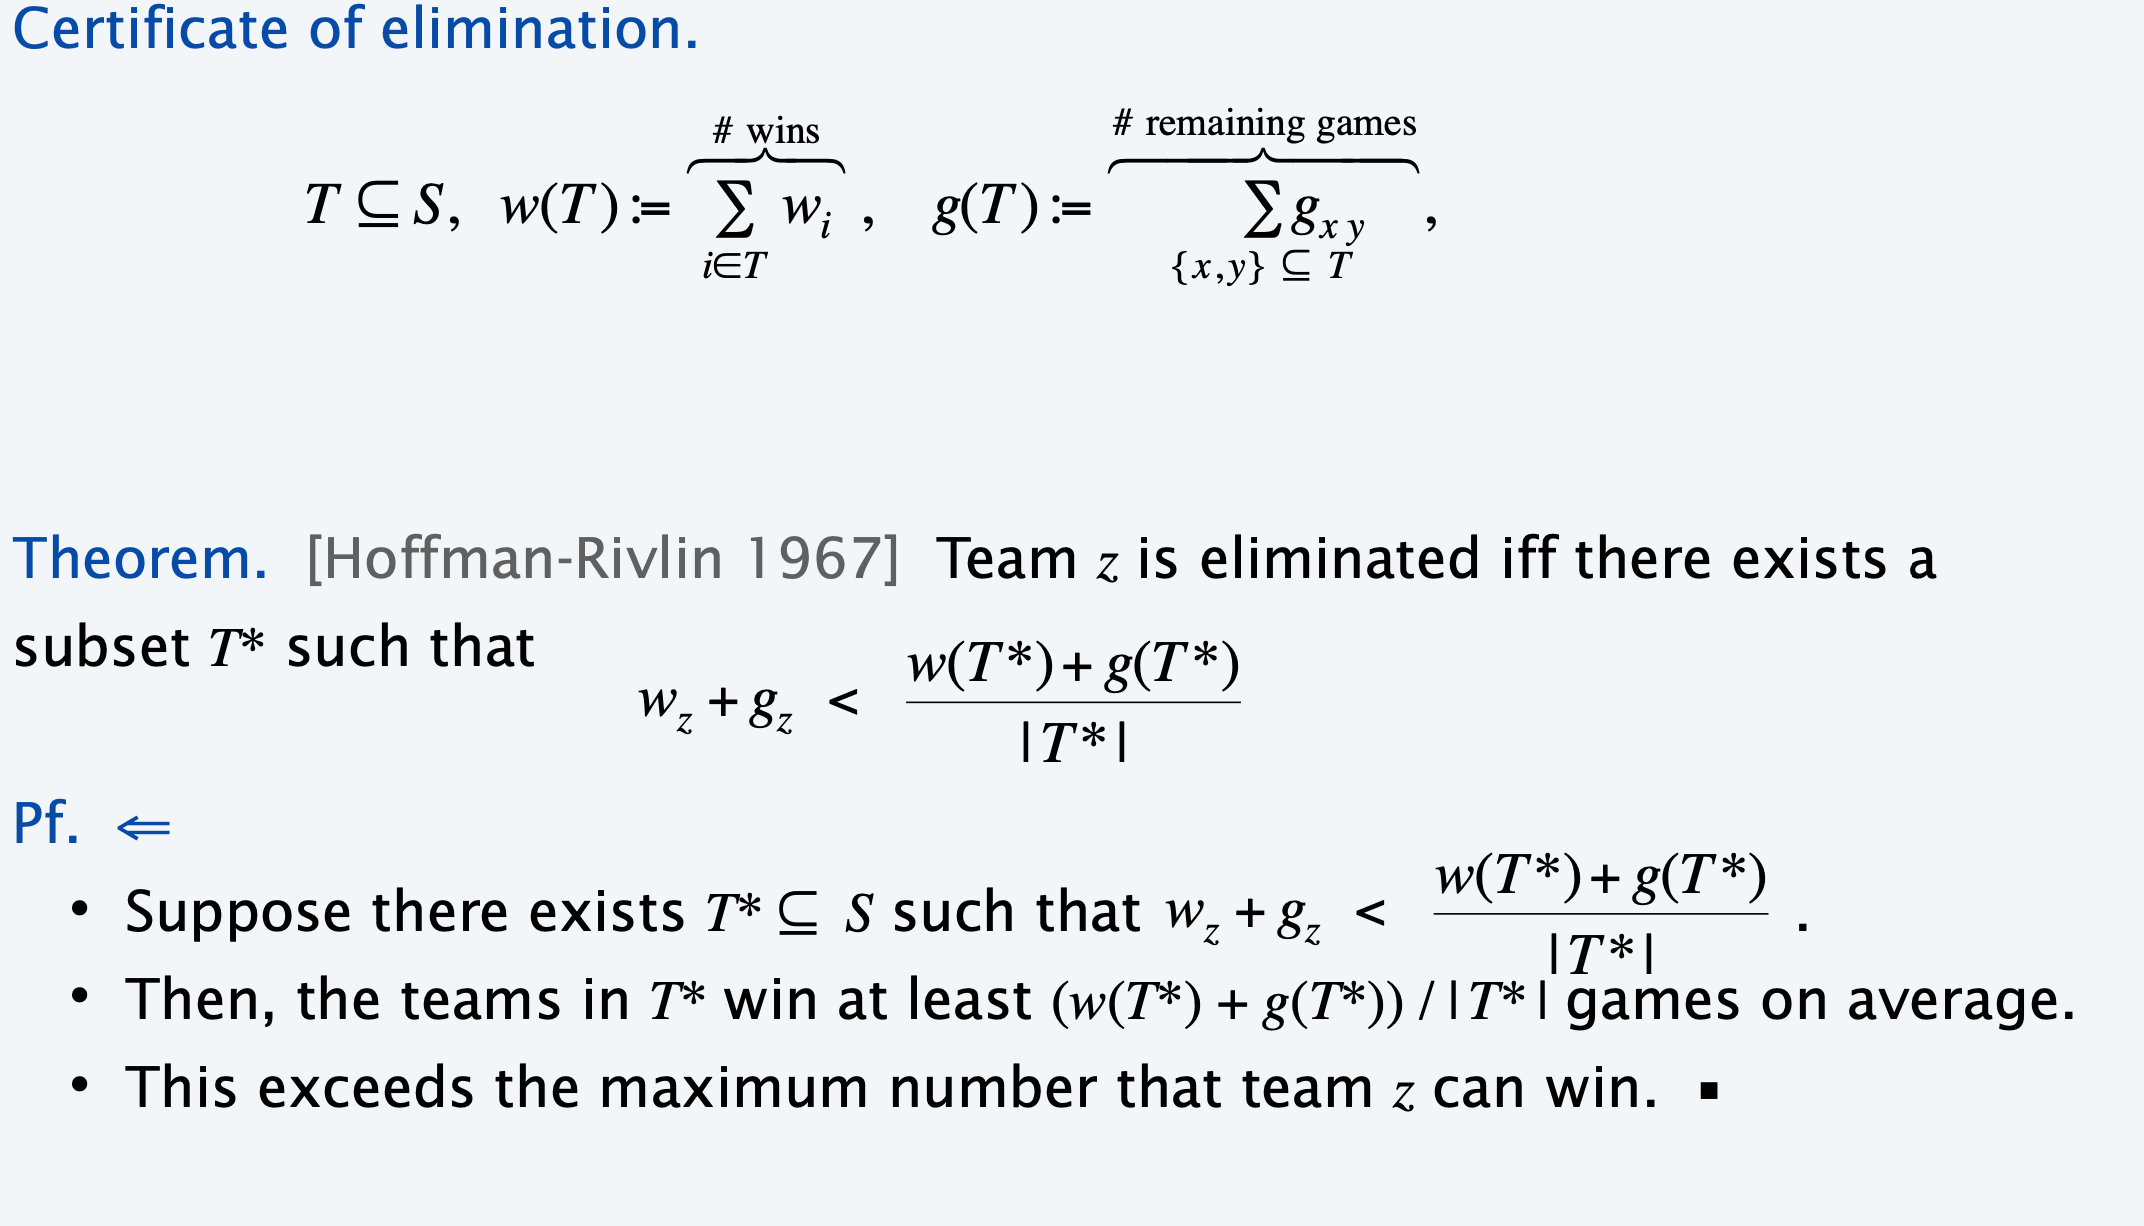
\includegraphics[width=0.6\textwidth ]{baseballElimination}
\end{figure}

\end{document}
